\documentclass{class/thesisclass}
% Based on thesisclass.cls of Timo Rohrberg, 2009

%% ---------------------------------
%% | Information about the thesis  |
%% ---------------------------------

% Possible titles:
% Three parts: A and B C
%  Part A:
%   - Track Finding in the Central Drift Chamber and
%   - Improvements on the Track Finding and
%   - Improvements on the Track Finding in the Central Drift Chamber and
%   - Combination of a Local and a Global Track Finder and
%  Part B:
%   - Momentum Estimation of Slow Pions
%   - Momentum Estimation of Slow Pions with the Energy Loss
%   - Momentum Estimation of Slow Pions with the Deposited Energy
%   - Momentum Estimation of Slow Pions in the Vertex Detector
%  Part C:
%   - for the Belle~II Experiment

\newcommand{\myname}{Nils Braun}
\newcommand{\mytitle}{Momentum Estimation of Slow Pions and Improvements on the Track Finding in the Central Drift Chamber for the Belle~II Experiment}
\newcommand{\mytitlegerman}{Impulsbestimmung langsamer Pionen und Verbesserungen der Spurfindung in der zentralen Driftkammer für das Belle~II Experiment}
\newcommand{\myinstitute}{Institut für experimentelle Kernphysik (IEKP)}
\newcommand{\myinstituteen}{Institut of Experimental Nuclear Physics (IEKP)}

\newcommand{\reviewerone}{Prof. Dr. Michael Feindt}
\newcommand{\reviewertwo}{Prof. Dr. Ulrich Husemann}

\newcommand{\timestart}{November 2014}
\newcommand{\timeend}{November 2015}
\newcommand{\submissiontime}{11. November 2015}

\newcommand{\iekpnumber}{2015-20}

%% -------------------------------
%% |  Information for PDF file   |
%% -------------------------------
\hypersetup{
	pdfauthor={Nils Braun},
	pdftitle={\mytitle},
	pdfsubject={},
	pdfkeywords={Track, Finding, CDC, VXD, Slow, Pions, dEdX, Belle, Belle II, Japan, Segments, Tracks, Stereo, Drift Chamber, Vertex Detector, Combination, Fit, Momentum Estimation}
}


%% --------------------------------
%% | Settings for word separation |
%% --------------------------------
% Help for separation:
% In german package the following hints are additionally available:
% "- = Additional separation
% "| = Suppress ligation and possible separation (e.g. Schaf"|fell)
% "~ = Hyphenation without separation (e.g. bergauf und "~ab)
% "= = Hyphenation with separation before and after
% "" = Separation without a hyphenation (e.g. und/""oder)

% Describe separation hints here:
\hyphenation{
} 


\LetLtxMacro{\oldtodo}{\todo}
\renewcommand{\todo}[2][]{\oldtodo[inline, #1]{#2}}

% Listen
\newcounter{RRR}
\newenvironment{Rlist}{
  \begin{list}{(\Roman{RRR})}{
      \usecounter{RRR}\setlength{\leftmargin}{8mm}\setlength{\labelsep}{2mm}
    }
}{\end{list}}

\newcounter{rrr}
\newenvironment{rlist}{
  \begin{list}{(\roman{rrr})}{
      \usecounter{rrr}\setlength{\leftmargin}{8mm}\setlength{\labelsep}{2mm}
    }
}{\end{list}}

\newcounter{zzz}
\newenvironment{zlist}{
  \begin{list}{(\arabic{zzz})}{
      \usecounter{zzz}\setlength{\leftmargin}{8mm}\setlength{\labelsep}{2mm}
    }
}{\end{list}}

\newcounter{abc}
\newenvironment{alist}{
  \begin{list}{(\alph{abc})}{
      \usecounter{abc}\setlength{\leftmargin}{8mm}\setlength{\labelsep}{2mm}
    }
}{\end{list}}

% Mathematische Symbole
\newcommand{\nM}{\mathbb}
\newcommand{\nR}{\mathbb{R}}
\newcommand{\nN}{\mathbb{N}}
\newcommand{\nZ}{\mathbb{Z}}
\newcommand{\nQ}{\mathbb{Q}}
\newcommand{\nC}{\mathbb{C}}
\newcommand{\nK}{\mathbb{K}}
\newcommand{\nF}{\mathbb{F}}
\newcommand{\nullel}{\mathcal{O}}
\newcommand{\einsel}{\mathds{1}}

\newcommand{\summe}[2]{\sum\limits_{#1}^{#2}}

\newcommand{\coss}[1]{\cos\left( #1 \right)}
\newcommand{\sinn}[1]{\sin\left( #1 \right)}
\newcommand{\psumme}{\sum\limits_{n=0}^{\infty}}


\newcommand{\limesn}{\lim\limits_{n\to\infty}}
\newcommand{\limesx}{\lim\limits_{x\to\infty}}
\newcommand{\limesp}[1]{\lim\limits_{#1\to\infty}}
\newcommand{\limespfeil}[1]{\xrightarrow[#1\to\infty]{}}
\newcommand{\limesto}[2]{\lim\limits_{#1 \to #2}}
\newcommand{\limes}[1]{\lim\limits_{#1}}
\newcommand{\limespfeilto}[1]{\xrightarrow[#1]{}}
\newcommand{\limesw}[1]{\xrightarrow[#1]{W}}





\newcommand{\dd}[2]{\frac{\mathrm d#1}{\mathrm d#2}}
\newcommand{\pp}[2]{\frac{\partial#1}{\partial#2}}
\newcommand{\ddx}{\frac{\mathrm d}{\mathrm dx}}
\newcommand{\ddt}[1]{\frac{\mathrm d #1}{\mathrm dt}}
\newcommand{\ddn}[2]{\frac{\mathrm{d}^{#2}}{\mathrm{d}#1^{#2}}}
\newcommand{\ddxn}[1]{\frac{\mathrm{d}^{#1}}{\mathrm{d} x^{#1}}}
\newcommand{\bint}[2]{\int\limits_{#1}^{#2}}
\newcommand{\aint}[1]{\int\limits_{#1}^{}}
\newcommand{\intd}{\ \mathrm d}
\renewcommand{\div}{\text{div }}
\newcommand{\rot}{\text{rot }}

\newcommand{\diag}[1]{\mathrm{diag}\left(#1\right)}

\newcommand{\LL}{\mathcal{L}}

\newcommand{\grad}{\text{grad} \ }

% for double arrows a la chef
% adapt line thickness and line width, if needed
%\tikzstyle{vecArrow} = [thick, ->, >=stealth,
%   double distance=7pt, shorten >= 5.5pt,
%   postaction = {draw,line width=7pt, white,shorten >= 4.5pt}]
\tikzstyle{vecArrow} = [thick, ->, >=stealth]

\tikzstyle{module} = [rectangle, draw, fill=kit-green50, 
      text width=8em, text centered, rounded corners]
\tikzstyle{module-background} = [rectangle, draw, fill=kit-green15, rounded corners]
      
\tikzstyle{cloud} = [draw, ellipse,fill=red!20, node distance=3cm,
      minimum height=2em]
\tikzstyle{tracks} = [draw, -latex']
\tikzstyle{hits} = [draw=red!60, -latex', fill=red!60]

\tikzset{ header node/.style = {
    text depth    = +0pt,
    fill          = white,
    draw},
  header/.style = {%
    inner ysep = +1.5em,
    append after command = {
      \pgfextra{\let\TikZlastnode\tikzlastnode}
      node [header node] (header-\TikZlastnode) at (\TikZlastnode.north) {#1}
    }
  }
}

\lstdefinestyle{customP}{
  belowcaptionskip=1\baselineskip,
  breaklines=false,
  %frame=L,
  xleftmargin=\parindent,
  language=Python,
  showstringspaces=false,
  basicstyle=\footnotesize\ttfamily,
  keywordstyle=\bfseries\color{kit-green70},
  commentstyle=\itshape\color{kit-blue70},
  identifierstyle=\color{black},
  stringstyle=\color{kit-orange100},
}

\lstdefinestyle{customC}{
  belowcaptionskip=1\baselineskip,
  breaklines=false,
  %frame=L,
  xleftmargin=\parindent,
  language=C++,
  showstringspaces=false,
  basicstyle=\footnotesize\ttfamily,
  keywordstyle=\bfseries\color{kit-green70},
  commentstyle=\itshape\color{kit-blue70},
  identifierstyle=\color{black},
  stringstyle=\color{kit-orange100},
}

\definecolor{light-gray}{gray}{0.98}

% the space reserved between for the ``In'' numbers and the code
% after http://tex.stackexchange.com/questions/223465/ipython-notebook-cells-with-listings
\newlength\inwd
\setlength\inwd{1.6cm}

\newcounter{ipythcntr}

\newtcblisting{inputipynb}[1][\theipythcntr]{
  enlarge left by=\inwd,
  width=\linewidth-\inwd,
  enhanced,
  boxrule=0.2pt,
  colback=light-gray,
  listing only,
  listing options={
    style=customP
  },
  top=-6pt,
  bottom=-6pt,
  left=4pt,
  overlay={
    \node[
      anchor=north east,
      text width=\inwd,
      font=\footnotesize\ttfamily\color{kit-blue100},
      inner ysep=2mm,
      inner xsep=0pt,
      outer sep=0pt
      ] 
      at (frame.north west)
      {\stepcounter{ipythcntr}In [#1]:};
  }
}

\newtcblisting{outputipynb}[1][\theipythcntr]{
  enlarge left by=\inwd,
  width=\linewidth-\inwd,
  enhanced,
  boxrule=0pt,
  frame hidden,
  colback=white,
  listing only,
  listing options={
    basicstyle=\footnotesize\ttfamily,
  },
  top=-6pt,
  bottom=-6pt,
  left=4pt,
  overlay={
    \node[
      anchor=north east,
      text width=\inwd,
      font=\footnotesize\ttfamily\color{kit-blue100},
      inner ysep=2mm,
      inner xsep=0pt,
      outer sep=0pt
      ] 
      at (frame.north west)
      {Out [#1]:};
  }
}


\begin{document}

  %Titelseite und Inhaltsverzeichnis
  \pagenumbering{alph}
  \frontmatter
  \pagenumbering{Roman}
  % coordinates for the bg shape on the titlepage
\newcommand{\diameter}{20}
\newcommand{\xone}{-15}
\newcommand{\xtwo}{160}
\newcommand{\yone}{15}
\newcommand{\ytwo}{-253}

\newgeometry{top=5cm,left=5.5cm, right=0cm}

\begin{titlepage}
% bg shape
  \begin{tikzpicture}[overlay]
    \draw[color=gray] (\xone mm, \yone mm) -- (\xtwo mm, \yone mm) arc (90:0:\diameter pt) -- (\xtwo mm + \diameter pt , \ytwo mm) -- (\xone mm + \diameter pt , \ytwo mm) arc (270:180:\diameter pt) -- (\xone mm, \yone mm);
  \end{tikzpicture}
  \begin{textblock}{10}[0,0](4,2.5)
    
\includegraphics[width=.3\textwidth]{logos/KITLogo_RGB.pdf}
  \end{textblock}
  \changefont{phv}{m}{n} % helvetica
  \begin{textblock}{10}[0,0](6.0,2.85)
    \hfill \textsc{IEKP-KA/2015-??}
  \end{textblock}
  \vspace*{2.3cm}
  \begin{center}
    \begin{minipage}{10cm}\centering\huge{\mytitle}\end{minipage}\\
    \vspace*{0.9cm}
    \Large{\myname}\\
    \vspace*{2cm}
    \Large{Masterthesis}\\
    \vspace*{1cm}
    \Large{\submissiontime}\\
    \vspace*{1cm}
    \Large{\myinstituteen}
  \end{center}
  \vspace*{2.5cm}
  \Large{
    \begin{center}
    \begin{tabular}[ht]{l c l}
      Advisor: & \hfill  & \reviewerone\\
      Coadvisor: & \hfill  & \reviewertwo
    \end{tabular}
    \end{center}
  }
  \vspace*{0.5cm}
  \begin{center}
    \large{Editing time: \hspace*{0.01cm} \timestart \hspace*{0.25cm} -- \hspace*{0.25cm} \timeend}
  \end{center}
  \begin{textblock}{10}[0,0](4,16.8)
    \tiny{KIT -- Universit\"at des Landes Baden-W\"urttemberg und nationales Forschungszentrum in der Helmholtz-Gemeinschaft}
  \end{textblock}
  \begin{textblock}{10}[0,0](14,16.75)
    \large{\textbf{www.kit.edu}}
  \end{textblock}
\end{titlepage}

\newpage
\thispagestyle{empty}
\mbox{}

\begin{titlepage}
% bg shape
  \begin{tikzpicture}[overlay]
    \draw[color=gray] (\xone mm, \yone mm) -- (\xtwo mm, \yone mm) arc (90:0:\diameter pt) -- (\xtwo mm + \diameter pt , \ytwo mm) -- (\xone mm + \diameter pt , \ytwo mm) arc (270:180:\diameter pt) -- (\xone mm, \yone mm);
  \end{tikzpicture}
  \begin{textblock}{10}[0,0](4,2.5)
    
\includegraphics[width=.3\textwidth]{logos/KITLogo_RGB.pdf}
  \end{textblock}
  \changefont{phv}{m}{n} % helvetica
  \begin{textblock}{10}[0,0](6.0,2.85)
    \hfill \textsc{IEKP-KA/2015-??}
  \end{textblock}
  \vspace*{2.7cm}
  \begin{center}
    \begin{minipage}{10cm}\centering\huge{\mytitlegerman}\end{minipage}\\
    \vspace*{1cm}
    \Large{\myname}\\
    \vspace*{2cm}
    \Large{Masterarbeit}\\
    \vspace*{1cm}
    \Large{\submissiontime}\\
    \vspace*{1cm}
    \Large{\myinstitute}
  \end{center}
  \vspace*{3cm}
  \Large{
    \begin{center}
    \begin{tabular}[ht]{l c l}
      Referent: & \hfill  & \reviewerone\\
      Korrefferent: & \hfill  & \reviewertwo
    \end{tabular}
    \end{center}
  }
  \vspace*{0.5cm}
  \begin{center}
    \large{Editing time: \hspace*{0.01cm} \timestart \hspace*{0.25cm} -- \hspace*{0.25cm} \timeend}
  \end{center}
  \begin{textblock}{10}[0,0](4,16.8)
    \tiny{KIT -- Universit\"at des Landes Baden-W\"urttemberg und nationales Forschungszentrum in der Helmholtz-Gemeinschaft}
  \end{textblock}
  \begin{textblock}{10}[0,0](14,16.75)
    \large{\textbf{www.kit.edu}}
  \end{textblock}
\end{titlepage}

\restoregeometry
\cleardoublepage

  \vspace*{32\baselineskip}
\hbox to \textwidth{\hrulefill}
\par
Ich versichere wahrheitsgemäß, die Arbeit selbstständig angefertigt, alle benutzten Hilfsmittel vollständig und genau angegeben und alles kenntlich gemacht zu haben, was aus Arbeiten anderer unverändert oder mit Abänderungen entnommen wurde.

\textbf{Karlsruhe, \submissiontime}
\vspace{1.5cm}

\dotfill\hspace*{8.0cm}\\
\hspace*{2cm}(\textbf{Nils Braun}) %center name with hspace


\thispagestyle{empty}

\clearpage

\vspace*{35\baselineskip}
Masterarbeit angenommen.

\textbf{Karlsruhe}
\vspace{1.5cm}

\dotfill\hspace*{8.0cm}\\
\hspace*{1cm}(\textbf{\reviewerone}) %center name with hspace


\thispagestyle{empty}
\cleardoublepage

  \tableofcontents

  % Hauptteil
  \mainmatter

  \chapter{Introduction}

The Standard Model of particle physics (SM) is one of the most successful and precise theories developed in physics as it can describe observed phenomena over a large energy range (\cite{omg}, \cite{hydrogen}) with unrivaled precision~\cite{mu}. The theoretical foundations could only be developed and tested by the accurate measurements performed in the particle physics experiments all over the world. One of these experiments was the former Belle experiment in Tsukuba, Japan, which was used to measure important parts of the SM with high precision. 

However, there are many experiments which indicate that the SM is not the definite theory for particle physics. Examples are the observations of rotational velocities of galaxies \cite{galaxy} which can be explained by introducing the weakly interfering, invisible ``dark matter''. Not much is known about this new type of matter which is not part of the SM -- especially not their interactions with other particles or their characteristics like mass or spin. Another example is the imbalance between the observed matter and antimatter in the universe, which can be described by barion number violation, C and CP violation and thermal inequalities in the early universe \cite{sakharov}. Although there is theoretically well-understood CP violation in the SM, which was for example observed at the Belle experiment, this CP violation can not sufficiently create a matter--antimatter asymmetry of the measured size. Additionally, there are many candidates for new models beyond the SM like supersymmetry or string theory, which can describe the deviations from the SM or at least parts of it. Those theories introduce new particles that can already be observed by their impact on the interactions between the SM particles if these interactions are measured precisely enough.

Therefore the successor experiment -- Belle~II -- was planed and is currently being constructed to replace most of the Belle detector. It is built with advanced measuring devices and will be used to record a larger number of $\PB$ mesons -- the successor of the $\Pep\Pem$-collider (SuperKEKB) is planed to have an instantaneous luminosity 40 times higher than that of KEKB. The produced $\PB$ mesons decay further and by measuring the characteristics of the decay products like their momentum or their type one can draw conclusions on the primary, high energetic process.

% \begin{figure}
%   \centering
%   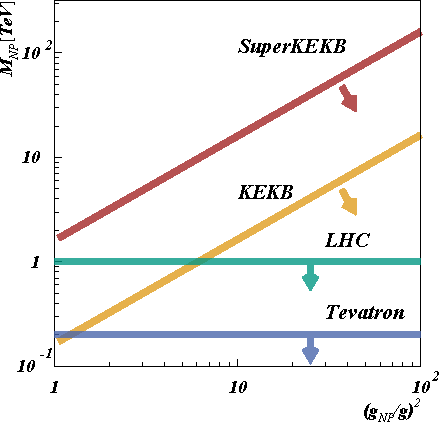
\includegraphics[width=0.6\linewidth]{figures/general/luminosity.pdf}
%   \caption{\cite{tdr}}
% \end{figure}

One of the key elements for measuring the decay products in the Belle~II experiment are the tracking detectors~\cite{tdr}. Their function is to detect the produced particles as well as to quantify their trajectory parameters, e.g.\ their momentum. To serve this purpose, space-resolved measuring devices in a homogeneous magnetic field are used to detect the locations of points on the curled trace of the charged particles through the detector, so-called hits. As there is no way to obtain information on which particle has produced which hit, this decision has to be made by algorithms implemented in software afterwards. These algorithms are called track finders and work with procedures comparable to pattern recognition tasks as they use the typical shape of the tracks in the detector to partition the hits. They output exclusive sets of hits which were possibly created by the same particle to the next step -- the track fitter~\cite{genfit} -- which determines the parameters of the trajectory.

As the tracking detectors are the only detector part with the task to find and measure all charged decay products, it is very important to find as many tracks as possible. High energy losses of the particles or multiple scattering with the detector elements can lead to deviations from the typical circular-shaped trajectory which can decrease the finding efficiency. Imperfections in the software and hits produced by beam-induced background (e.g.\ via secondary photon showers originating from scattered electrons or positrons) can lead to wrongly added hits or tracks and can deteriorate the resolution of the trajectory parameters calculated while fitting. Both figures of merit -- the finding efficiency and the number of incorrectly added hits and tracks -- can be improved by better approaches and refined algorithms in the tracking software.

Studies of rare decays use after the cuts typically only a small number of events~\cite{lutz} to perform their measurements, so loosing events because of a reduced finding efficiency can lead to crucial problems in these channels or could make it even impossible to analyze these decays. Also high-statistic studies performed with millions of events can be improved by a better tracking software, as the trajectory parameters go directly into the variables needed in the analyses and smaller errors on these parameters can improve the overall systematic uncertainty. As some analyses depend on the fact, that the whole event with all its measurements can be described consistently by a given model (by using variables as the measured energy still left in the detector after subtracting all reconstructed and classified particles~\cite{christian_phd}), the finding efficiency of the tracks together with a high purity plays a crucial part.

After an introduction into relevant parts of the Belle~II detector in chapter~\ref{chapter-ex}, the algorithms behind the track finders for the planned experiment as well as the calculated figures of merit will be described (chapter~\ref{chapter-theory}). The main part of this thesis will be dedicated to the improvements on the tracking software for the central drift chamber (CDC) -- the largest tracking detector of Belle~II. In chapter~\ref{chapter-workflow}, the newly developed algorithms together with their implementation will be described and evaluated. Among these algorithms is the hit finder for stereo hits, which are hits originating from sense wires with a small tilting angle that make it possible to determine the the trajectory along the beam direction. Compared to the old implementation, the results could be improved significantly by lowering the computing time drastically.

This thesis was the first to combine the two track finding algorithms, so a description of their characteristics and the algorithms for their combination will also be discussed in this chapter. The implemented changes could increase the number of correctly found tracks and hits significantly. Additionally, the number of wrong tracks and also the computing time of the whole algorithm could be decreased. During this thesis, the track finders could be enhanced to outperform the reference implementation copied from the Belle experiment for the first time in figures of merit as well as computing performance and the transition from this reference implementation to the newly developed track finders was made.

Pions with low momenta in the region of $\unit[50]{MeV} - \unit[100]{MeV}$ play an important role of many planned physics analyses. Because of their low momentum, they can not reach the CDC and can only be detected in the most inner detectors -- the vertex detectors (VXD). This however decreases their momentum resolution because of a smaller lever arm. To increase this resolution -- which is very important for the physics analyses -- again, another piece of information apart of the location of hits in the vertex detector is used: the energy loss per travel length. This value is connected to the momentum by the Bethe equation and can be used as input to the fitting routine~\cite{robert}. The newly developed procedure to use the momentum estimation of every hit separately, which could increase the number of successful fits as well as the momentum resolution drastically in the region $\unit[50]{MeV} - \unit[80]{MeV}$, will be described in chapter~\ref{chapter-vxd}.


  \chapter{Experimental Setup} \label{chapter-ex}
In the following sections the experimental setup for this thesis - the Belle II detector and the SuperKEKB collider - are described as far as it is necessary for the tracking software. Detailed information can be found elsewhere \cite{tdr}.


\section{SuperKEKB and the Belle II Detector}

The future Belle II is currently being build at the KEK high energy research facility in Tsukuba, Japan. It is a general purpose $4\pi$ detector for high energy particle experiments. A scheme of the whole detector with the planned measuring devices can be found in figure \ref{fig-belle2}.

\begin{figure}
 \centering
 \includegraphics[height=0.4\textheight]{figures/experimental_setup/detector_crossection_labels.pdf}
 \caption[Schema of the planned Belle II detector.]{Scheme showing the planned Belle II detector in top view. The single measuring devices are shown with their names. Some more information on the tracking devices can be found in the text. Taken from \cite{christian}.}
 \label{fig-belle2}
\end{figure}

\begin{figure}
 \centering
 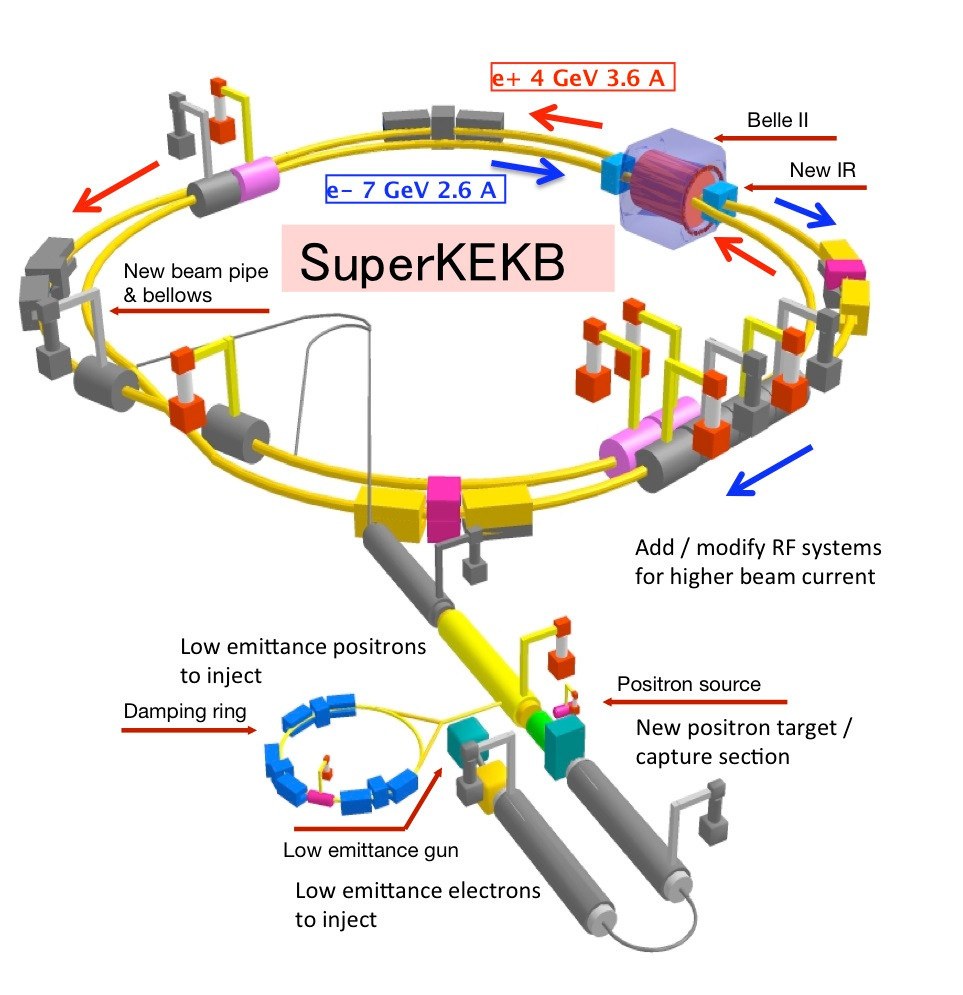
\includegraphics[height=0.4\textheight]{figures/experimental_setup/superkekb.jpg}
 \caption[Sketch showing the SuperKEKB electron-positron collider.]{Sketch showing the SuperKEKB electron-positron collider with the Belle II detector. Taken from \cite{DesyWebseite}.}
 \label{fig-superkekb}
\end{figure}


The Belle II detector is used for measuring the electron positron collisions induced by the two-ring asymmetric-energy SuperKEKB collider. A sketch of the collider can be found in figure \ref{fig-superkekb}. As its predecessor KEKB its center of mass energy is tuned in such a way that it lays near the $\PgUc$ resonance. This beam energy is chosen because a $\PgUc$ particle decays with a branching fraction of 96 \% into a pair of entangled B-mesons. As described in the introduction, the daughter particles of these B mesons open a window to a very wide range of physical studies like CP violation or meson spectroscopy. The energy of the colliding electrons and positrons is asymmetric which leads to a slightly asymmetric collision as well. This fact is exploited in measuring the decay length of the two formed B-Mesons - one of the main ingredients for quantifying the CP violation in the B-Meson system. 

The usage of electrons and their antiparticles for collisions leads to very clean events compared to other collision partners like protons or even gold atoms. Clean means in this context that a reduced number of created decay products (only 11 charged tracks on average) and no pile up (only one collision occurring at the same time) are expected. These circumstances can be used for high precision measurements on the formed particles.

As every general purpose high energy particle physics detector the Belle II detector is composed of several single measuring devices - each one with a different task. The detector consists of basically six measurement layers:
\begin{zlist}
  \item two layers of silicon pixel detectors for measuring the charged particles near the interaction point (PXD),
  \item another four layers of doubled-sided silicon strip layers (SVD),
  \item the central drift chamber (CDC) for measuring the momentum of charged particles,
  \item a time-of-propagation counter (TOP) together with the endcap particle identification detector (aerogel ring imaging Cherenkov detector) for identification of the produced particles using Cherenkov radiation,
  \item an electromagnetic calorimeter (ECL) build of scintillating CsI(Tl) crystals for measuring the energy of all electromagnetic interacting particles,
  \item and the longliving kaon and myon detector (KLM) identifying these particle types in the outer region of the detector to improve the overall particle identification.
\end{zlist}

\section{The Tracking Detectors}

For collecting many information on the physical process in the collision, many information on the created decay products are needed. These include
\begin{zlist}
 \item Identification of the created particles (for example by their mass),
 \item Measurement of the kinematic properties (like momentum and energy) of the charged particles,
 \item Resolution of their origin position - also called their vertex.
\end{zlist}

The tracking detectors described in this thesis are mainly build for recording the momenta of the particles as well as the position of their trajectories. The position information can then be further used for combining two or more particles which originate from the same particle for measuring the vertex position. %Further more special applications are identification of the particle type by their energy loss.

The measuring principle of the positions and also the momenta of charged decay products is to let the particles fly throw a sensor region with space-resolved measurement and obtain their full path through the detector - a so called track - by combining the different location information - the so called hits. By applying a magnetic field - in Belle II it has a nominal field strength of $B = \unit[1.5]{T}$ - parallel to the beam axis which is the $z$ axis in the coordinate system of the detector, the charged particles curl. By measuring the curvature of the curled tracks an estimation of the momentum in the plane perpendicular to the beam axis - the $r$-$\phi$-plane - can be made. The remaining $z$-direction parallel to the beam axis can be computed with the angle of the track to the beam axis\footnote{The coordinate system in Belle II is chosen as the typical one in high energy particle physics: The $z$-axis is parallel to the beam whereas the $x$- and $y$-axis span a plane perpendicular to the beam line. The origin is the interaction point. Most of the time, one uses $r = \sqrt{x^2 + y^2}$ and $\phi = \arctan(y/x)$ rather than $x$ and $y$ directly.}.

There exist many different ways to measure the position of a charged particle. Each of them exploits the charge of the particles and their interaction with materials which makes these techniques unusable for neutral particles. The vertex positions and momenta of uncharged particles can not be measured with the here presented methods. In Belle II the momenta of neutral particles are resolved by assuming momentum conservation or by measuring the total energy of the particles in the calorimeter\footnote{Photons for example are neutral particles but deposit energy in the electromagnetic calorimeter as well.}. In the following two tracking devices for charged particles are described in more detail. The main part (chapters \ref{chapter-theory}, \ref{chapter-workflow} and \ref{chapter-results}) of this thesis covers the tracking in the CDC detector. Only chapter \ref{chapter-vxd} on the VXD momentum estimation for slow pions handles the tracking in the VXD detectors.

\subsection{CDC}

CDC is an acronym for Central Drift Chamber and with its radius of about $\unit[1.3]{m}$ the largest tracking detector in Belle 2. The CDC is a typical gas chamber detector with 14336 sense wires arranged in 56 layer and 9 superlayers. These sense wires together with a much larger number of field wires are strained mostly parallel to the beam axis in a cylindrical tank flooded with gas which spreads the whole detector in $z$-direction. The gas is a mixture of 50 \% helium and 50 \% ethane. For more information on gas chamber detectors see for example \cite{grupen}.

Each charged particle produced in the collision of the electron and position with a transversal momentum high enough to exit the inner VXD detectors, interacts with the gas and can ionize the helium atoms. The energy deposit of a charged particle is given by the Bethe formula \cite{bethe}
\begin{align}
 - \left\langle \dd{E}{x} \right\rangle = \frac{4 \pi n z^2}{m_e c^2 \beta^2} \cdot \left( \frac{e^2}{4 \pi \varepsilon_0} \right)^2 \left[ \ln\left( \frac{2 m_e c^2 \beta^2}{I(1 - \beta^2} \right) - \beta^2 \right] \ , \label{form-bethe}
\end{align}
which describes the average energy loss per travel length. This energy is transfered to the shell electrons of the helium gas atoms. As the ionization energy of helium is very low (about $\unit[20]{eV}$) the helium atoms release their electrons very easily. These free electrons get accelerated in an electric field. This electric field is induced by applying a high voltage between sense and field wires. An instructive simulation of the typical electronic field distribution between 7 sense wires and 34 field wires can be found in figure \ref{fig-sense-wires}. The direction of the electric field is chosen that the field strength near the sense wires increases with $\propto 1/r$. The energy of the free electrons increases there rapidly so that they can ionize helium atoms by themselves as well. This whole ``flood'' of free charge can be detected by the electronics attaches to the sense wires and produce a sharp peak there. The more immobile helium atomic cores get absorbed later by the field wires. 

Because the free electrons have to drift through the gas, the measured peak has a delay up to $\unit[500]{ns}$ for the largest drift cells to the initial charged particle passage. By analyzing the time and location information of each measured peak, the path of the charged particle through the CDC can be reconstructed. A typical event display of the simulated passage of ten charged pions with $\unit[1]{GeV}$ can be seen in figure \ref{fig-event-display}. As the electric charge configuration in each drift cell is almost rotationally symmetric, there is no way to obtain information on the direction of the electron flood hitting the sense wire. Each wire produces a so called drift circle rather than a single hit point. These drift circles can also be seen in the figure.

If all CDC wires were strained perfectly parallel to the beam axis in $z$-direction, there would be no possibility to measure the $z$-information like the angle between the charged particles and the beam axis. That is the reason why some of the wires are installed with a small tilting angle to the beam axis\footnote{More correct is that these wires get twisted not tilted, but as the twisting angle is small, there is not much difference in the two descriptions.}. These wires are called stereo wires in contrast to the axial wires without tilting angle. A measured hit on the stereo wires alone does not give information neither on the position along the beam axis nor in the layer parallel to it as there is no possibility to measure the position along the wire where the particle passed by. Only the information collected among all axial and stereo hits lead to a correct estimation of the momentum in all directions as the axial wires define the position on the $r$-$\phi$-plane which in turn can be used to calculate the $z$-information with the stereo wires. A sketch of some axial and stereo wires sharing the same distance from the beam axis - also called a layer of wires - are shown in \ref{fig-axial-stereo}.

\begin{SCfigure}
  \caption{Simulation of the electron field in an extract of the wires in the central drift chamber. The violet circles depict the field wires whereas the red small points are the sense wires. The yellow paths are examples for the drift paths of ionized electrons. This simulation includes the distortion by the magnetic field. Taken from \cite{cdc_design}.}
  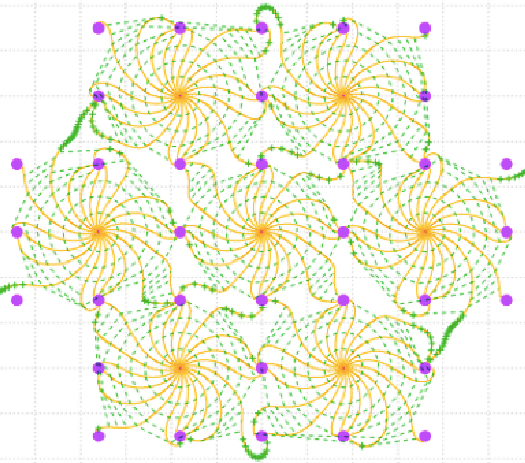
\includegraphics[width=0.5\linewidth]{figures/experimental_setup/electronsInCDC.pdf}
  \label{fig-sense-wires}
\end{SCfigure}


\begin{figure}
  \centering
  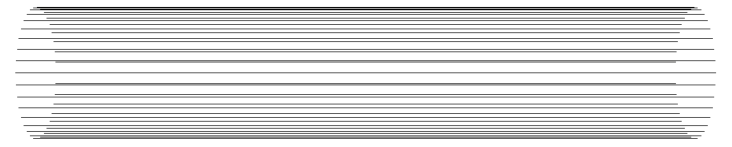
\includegraphics{figures/experimental_setup/axialLayers.pdf}
  
  \vspace*{1.5cm}
  
  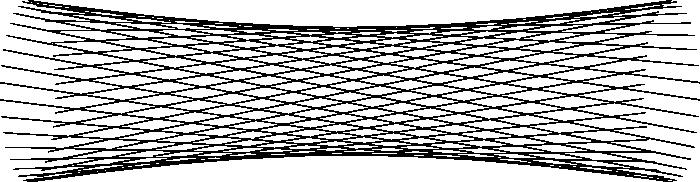
\includegraphics{figures/experimental_setup/stereoLayers.pdf}
  \caption{Drawing sketching the axial (top) and stereo wires in the CDC. The skewing against the beamline of the stereo (bottom) wires is exaggerated. Taken from \cite{oliver}.}
  \label{fig-axial-stereo}
\end{figure}

\begin{figure}
  \centering
  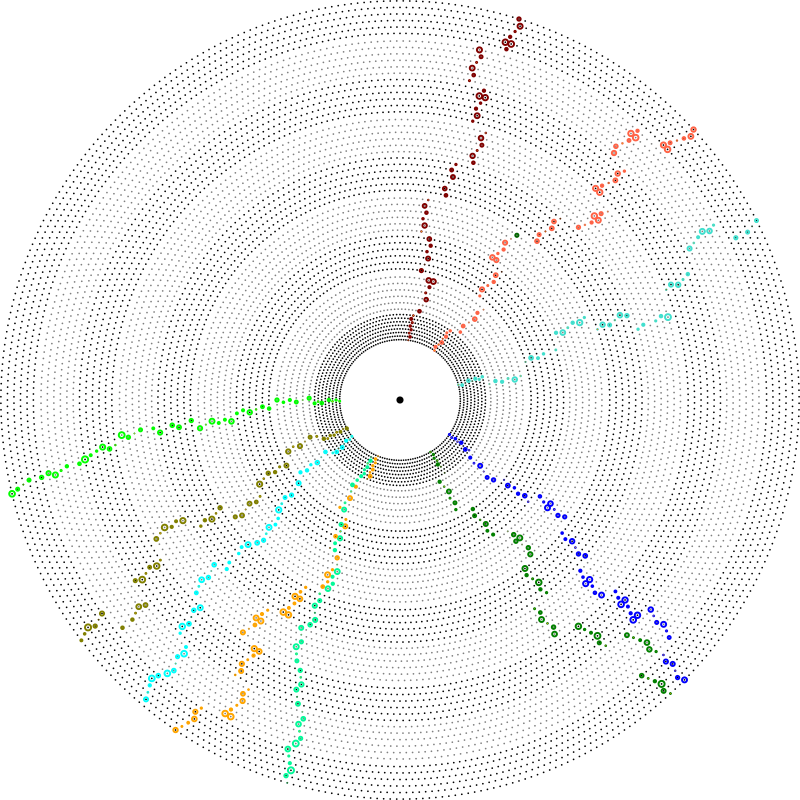
\includegraphics[width=0.8\linewidth]{figures/experimental_setup/eventDisplayPionGun.png}
  \caption{Simulated event of the passage of 10 $\Ppi^\pm$ with approximately $\unit[1]{GeV}$ through the CDC shown in a plane perpendicular to the beam axis. The interaction point is drawn as a black circle in the center. Each particle is colored differently to distinguish between them. Only the CDC detector is shown for better visibility. The wires are shown as gray (stereo) or black (axial) points. The hit wires are depicted with their drift circles. The appearing disruption in the circular paths of the particle arise due to the tilting angle of the stereo wires in respect to the axial wires.}
  \label{fig-event-display}
\end{figure}

\subsection{VXD}
VXD stands for vertex detectors and describes a group of two sorts of detectors: the pixel vertex detector (PXD) and the strip vertex detector (SVD). These two detectors are the innermost tracking detectors and are therefore used for measuring low momentum particles that do not reach into the CDC and the vertex positions of all produced decay products. 

The PXD consists of two layers of over eight million depleted field effect transistor pixels made of silicon. Because of their large number the occupancy is below 1 \% so their long readout time of over $\unit[20]{\mu s}$ can be handled better. \todo{size, form -> later, describe measurement system, describe energy loss -> later} 

The SVD is build of 4 layers of double-sided silicon strips todo{size, form -> later}. Its measurement system is comparable to the pixel detectors described before. As it can be seen in figure \ref{fig-belle2} the strips in the forward direction of the detector are constructed with a small slope of about $15^\circ$ because in this direction the bigger part of the decay products is expected. The found tracks in the SVD can be used to connect the results from the CDC and the PXD. Also because of the much smaller readout time in the SVD one can use it to improve the tracking in the pixel detector. 

  \chapter{Track Finder Theory and Multivariate Classification}

Before explaining the implemented changes to the track finder for the Belle II experiment in more detail, the principles of the Belle II software framework are explained briefly. More information can be found elsewere \todo{quote}. Afterwards common figures of merit for all track finders are explained and discussed and the working principles of the already implemented track finders are illustrated. 

\section{The Belle II Analysis Framework (\texttt{basf2})}

For simulation, data acquisition, data processing and analysis of the Belle II experiment the Belle Analysis Software Framework 2 (\texttt{basf2}) is used. Although - guided by its name - it seems to be build on top of the old software framework used for the Belle experiment it is a complete rewrite of the software using modern programming principles in the coding languages C++ \cite{cpp} and Python 2.7 \cite{python}. Together with external programming libraries like ROOT \cite{root} or EvtGen \cite{evtgen} that are already on the market this framework builds the base for every software written for the experiment.

The software is divided into several packages - each serving a single purpose or summarizing code for a single detector. Examples for the packages are CDC, SVD or the tracking packaged which is described in more detail in later chapters.

Each usage of the Belle Analysis Software Framework - if it is either a simulation, a reconstruction or an analysis does not matter - consists of processing one or more so called \emph{paths} build with \emph{modules}. These modules perform a dedicated small task like simulating the hard scattering event (the so called \texttt{EvtGen} module), writing out data to a root file (the module is called \texttt{RootOutput}) or performing a track reconstruction (for example with the module \texttt{TrackFinderCDCAutomaton}). The presence, the order and the parameters of the modules are determined in \emph{steering} files written with python. The modules itself can be written in C++ or python. 

In these steering files a path is created, filled and passed to the framework which handles loading the corresponding C++ libraries and calling the modules for every event that should be processed. An example of a small steering file for track finding can be found in listing \ref{lis-steering-file}. \todo{listing} Caused by this extremely modular structure not only parallel processing but also debugging of intermediate steps can be performed much easier.

Because many modules need the data produces by other modules before there is a need for intermodular communication. This communication is performed within the framework with the help of the data store. This class as a wrapper around a collection of named \texttt{TClonesArrays} from the ROOT library \cite{tclonesarray} which can store lists of instances of nearly arbitrary C++ classes. It is used widely in the framework to store all sorts of things like the hit information produced by the particles in the simulation or the found tracks after the track finding modules. The modules have read and write access to every so called store array in the data store. A visualization of the data flow between the modules created with the steering file in \ref{lis-steering-file} can be found in figure \ref{fig-viz-datastore}. The data store can be written to or read from disk using ROOTs own serialization mechanism together with data member dictionaries for the C++ classes created by the C++ interpreter of ROOT called CINT.

\section{Working Principle of the implemented CDC Track Finder in \texttt{basf2}}

One part of this work was the improvement and further development of the track finder modules for the CDC tracking detector. Therefore the working principles of the two track finder for this detector are described here briefly. For more information on the first track finder - the legendre track finder - see \cite{kronenbitter}. More information on the second described track finder - the automaton track finder - can be found in \cite{oliver}.

The general purpose of a track finder algorithm is to partition all measured wire hits into exclusive sets of hits that may come from the same charged particle passing through the detector. It does so by using several assumptions on the charged particle producing the wire hits like the form of their trajectory and therefore the possible patterns of the hits. After fitting a mathematical model of a trajectory to these hits one can gain information on the momentum or the vertex position of this particle. There are several different approaches to find the correct sets of hits which are in the following called tracks.

The reason to have two track finders for the CDC is their different ansatz. The legendre track finder is a so called global track finder whereas the automaton track finder is a local one. A global algorithm uses the information of all wire hits simultaneously. The legendre track finder does this by applying a mathematical projection to the wire positions which should in principle project all hits belonging to the same track onto the same coordinates. A local algorithm however tries to use neighboring wire hits to construct clusters of hits. These clusters are then enlarged by using neighborhood relations until a full track can be found. In the following these two principles are described in more detail.

\subsection{The Legendre Track Finder}
The principle of using the legendre transformation for tracking algorithms in high energy particle experiments was first described by Alexopoulos \cite{legendre}. It uses an extended version of the hough transformation introduced by Paul V.V. Hough in 1962. The algorithm uses the fact that each trajectory in the $r$-$\phi$-plane of the detector can be described by a circle - assuming no energy loss - because of the applied magnetic field. In a first approximation one can also assume that each particles comes from the interaction point which is valid for the bigger part of the decay products. Therefore the trajectory in the $r$-$\phi$ direction can be described by two parameters: the radius $R$ of the circle and the angle $\phi$ between an arbitrary but fixed axis and the tangent to the circle at the interaction point.

The idea is now to transform the $x$ and $y$ coordinate pair of every axial wire hit together with the drift length $R$ with the function
\begin{align*} x' = \frac{2x}{x^2 + y^2 - R^2} \qquad y' = \frac{2y}{x^2 + y^2 - R^2}  \qquad R' = \frac{2R}{x^2 + y^2 - R^2} \end{align*}
$$r = x' \cos(\theta) + y' \sin(\theta) \pm R'$$
into the legendre space as it can be seen in figure \ref{fig-legendre-explained}. In the first step, the wire hits are transformed to the inverted plane. With this transformation each circular trajectory through the interaction point is mapped onto a line going through the origin. After that each drift circle is transformed into a pair of sinusoidal functions. This function is constructed in that way to use the fact that each trajectory of a charged particle responsible for a wire hit must touch the drift circle tangentially. Each point on the constructed sinusoidal functions correspond to one possible trajectory of a particle which could have created such a hit. The coordinates in the legendre space are the two parameters describing the trajectory as mentioned before. There are two sinusoidal functions because the osculation point can be on the far or the near side of the drift circle - the trajectory circle can contain the drift circle or not.

With using the information of a single hit one ends up with an infinite number of trajectory hypothesis. But as a charged particle passed many drift cells until it leaves the CDC detector - in some cases up to 100 hits - several wire hits are created with the same trajectory parameters. As these same parameters correspond to the same point in the legendre space, the sinusoidal functions of the wire hits intersect in this point as it can be seen in figure \ref{fig-legendre-many}. The task of the legendre algorithm is now to do the transformation of the hit coordinates and find those intersections.

Imperfections due to energy loss and material effects make the sinusoidal function not interact in one single point but rather in smeared area. To copy with this problem but still find the intersections with a good performance a peak search in the legendre space is applied. The legendre space is divided into small bins. For each bin the number of sinusoidal functions passing this area is counted. The bin with the highest weight is assumed to be the bin with the highest number of sinusoidal intersections. From the wire hits contributing to this bin a new track is created and the search is repeated until a threshold in the bin entry is undercut. As the legendre space is mostly empty this procedure can be further improved in performance by refining the bin devision from very coarse bin sizes to finer ones only for those bins which have a certain amount of sinusoidal functions in them. Because these bins are divided into 4 subbins the concept is also called a quad tree search. The whole search is depicted in figure \ref{fig-quad-tree-seach}.

\subsubsection{Stereo Hit Finding}


\subsection{The Automaton Track Finder}
Clusterizer, Automaton-Principle


\section{The used Figures Of Merit}

For testing and developing and also for later usage in the experiment setup we need to compile numbers from the implemented track finder algorithms to show how well they work. There are three different classes of figures of merit to describe a track finder. All three classes listed here are described in more detail below. The three classes are:
\begin{itemize}
  \item the efficiency (like the hit efficiency or the finding efficiency, also split up for different particle types, momentum regions or areas in the detector)
  \item the error rate (like the clone or fake rate)
  \item the computational performance (like timing and memory consumption)
\end{itemize}

The last class should be quite clear and is measured by the basf2-own measuring algorithms. As the tracking is part of the online reconstruction and may be once adopted for the high level trigger, the timing performance is very important. 

The other two classes can best be described with the algorithm how they get computed. It starts with a full Monte Carlo simulation of generic BB events with the full detector simulation afterwards. The created hits can then be parted into distinct sets - each describing a simulated tracks, called MCTrackCand (they are called track candidates to fit the naming convention of the track finder). Only those tracks are kept as a MCTrackCand, that have at least 3 hits in the CDC - otherwise they can not be fitted and even if there were a chance to find them via track finding, they could not be used for physics. After that, the simulated hits with the stripped MC information are used for track finding with the method to be evaluated. This can be done easily as the simulated hits are transformed in a format that is similar to the format that will be used later for the data coming from the experiment. After the track finder has produced a list of track candidates also, we can use the saved MC information to match tracks from the track finder to tracks from the mc algorithm (also called MC track finder) by counting the number of hits they share. The different cases are depicted and described in table \ref{tab-mc-track-finder}.

\begin{table}
  \begin{tabular}{m{0.4\linewidth}m{0.55\linewidth}} \toprule
    \centering 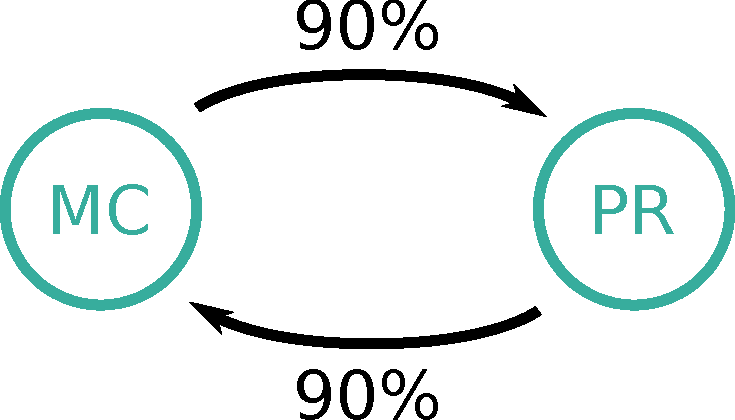
\includegraphics[width=0.8\linewidth]{figures/theory/fom_found.pdf} & There is a one to one connection between a MCTrackCand and a track from the track finder. The MCTrackCand is labeled found and the other track is labeled matched. \\ \midrule
    \centering 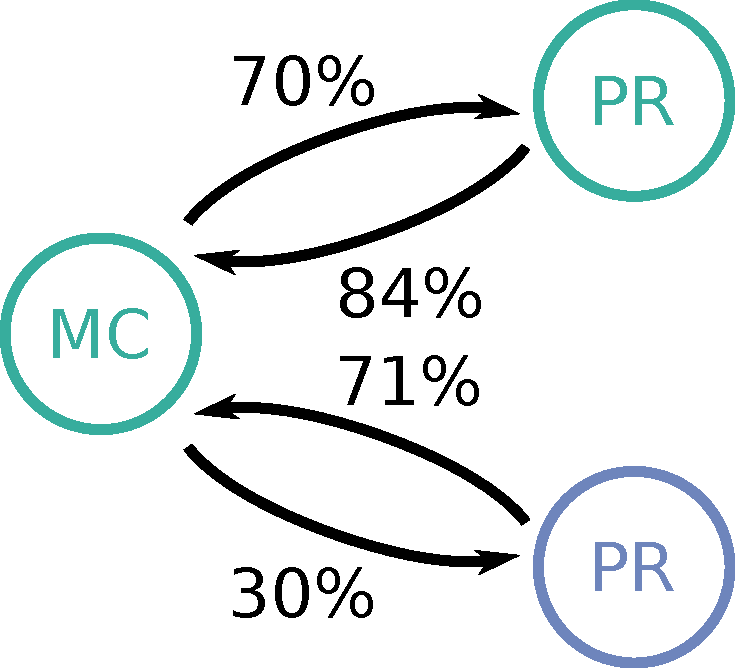
\includegraphics[width=0.8\linewidth]{figures/theory/fom_clone.pdf} & The MCTrackCand is found twice. The track from the track finder with the higher percentage (the green one in this example) is labeled matched, the other one cloned. The MCTrackCand is nevertheless labeled found. \\  \midrule
    \centering 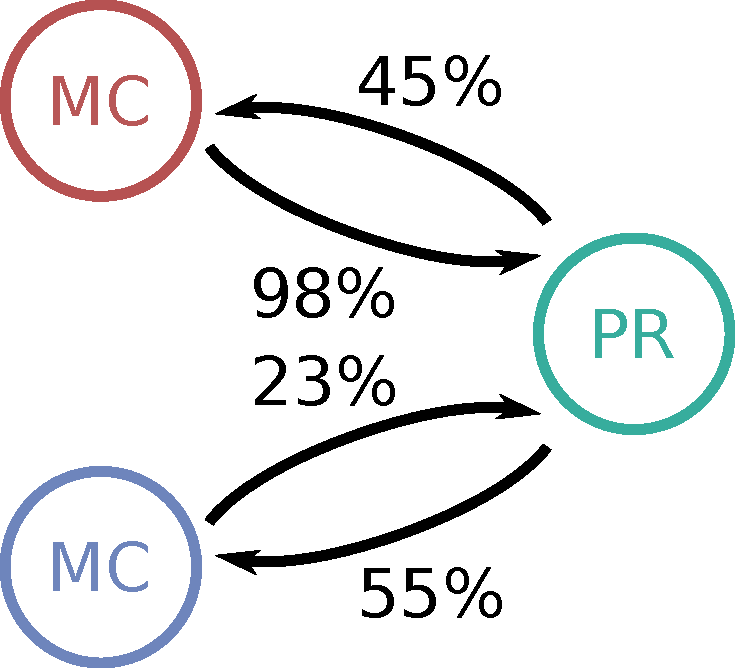
\includegraphics[width=0.8\linewidth]{figures/theory/fom_fake.pdf} & The track from the track finder is created with hits from many different MCTrackCands. As none of the corresponding hit ratios exceeds 66 \%, the track is called fake. There is no precise reason why the number 66\% was chosen. The hit ratios of the MCTrackCands itself do not play any role here. TODO: Is found for MC possible? \\  \midrule
    \centering 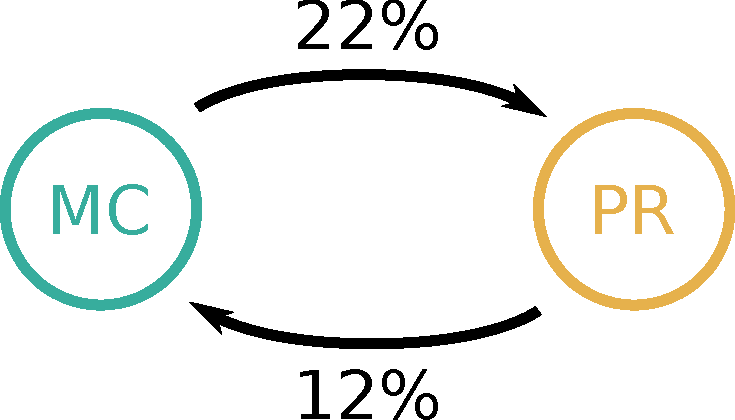
\includegraphics[width=0.8\linewidth]{figures/theory/fom_background.pdf} & The found track does not describe any of the MCTrackCands well (or well enough) - but is made out of background hits. This track is also called a fake. \\ \bottomrule
  \end{tabular}
  \caption[Matching routine for compiling the FOM.]{This tabular shows the four different cases for the matching between tracks found by the track finder (on the left side of the pictures) and MCTrackCands (shown on the right side). The different colors differentiate between different tracks. The connection between tracks shows that these two tracks share hits. The two percentages on the arrows are the percentages of hits they share in respect to the total number of hits in the MCTrackCand/track candidate from the track finder.}
  \label{tab-mc-track-finder}
\end{table}

The finding efficiency now describes the rate of MCTrackCands which are labeled matched by their total amount. Building this ratio can also be done for bins in various variables, like perpendicular momentum ($p_T$), angle in the curling plane ($phi$), number of tracks per event (multiplicity) and many more. A perfect track finder would have a finding efficiency of 100 \%. In most of the cases, the finding efficiency drops for tracks in a certain region of these variables - like for low momentum tracks.
The hit efficiency is the mean of the ratios between the number of hits in the MCTrackCands matched to a non-fake track candidate to the number of hits in total to this track. Here also a perfect track finder would have a hit efficiency of 100 \%. As in most of the cases the track finder looses some outlaying hits the hit efficiency drops.
The fake and clone rates are just the number of track candidates labeled as fake or clone by the matching algorithm divided by the number of found tracks in total. A perfect track finder would have both number set to 0 \%. A high fake rate is caused by a track finder with too loose cuts when putting together single pieces of tracks to a big track or by one which picks up background hits often. A track finder with a high clone rate on the other hand has to harsh cuts and splits up tracks into more than one piece.


\section{Multivariate Classification}
Classification, BDTs
  \chapter{Track Finding in basf2} \label{chapter-workflow}

After having described the principle of the track finders implemented in basf2 in the previous chapters, the actual changes to the software implementation during this thesis are discussed in this chapter. Before going into detail, the figures of merit of the two track finders showing their advantages and drawbacks are presented in the first section. After a short introduction in the general structure, the newly implemented background hit finder and the performed improvements on the stereo Legendre track finder are shown. Then the newly written \texttt{SegmentTrackCombinerModule} is described. The chapter ends with a section on general tools how to improve the found track candidates and an outlook.

All the plots showing recent results are done with the svn revision 21586.

\section{FOM of the two track finders}

\todo{TRASAN??}

Standalone legendre + standalone local
Legendre (old!): Finding efficiency, d0 influence, purity
Local: Segment purity, Finding efficiency; Clone + Fake-Rate of both track finder (Local with combined Segments)
Timing.

\todo{pictures: Finding efficiency legendre over pt, d0 influence, purity as histogramm}
\todo{pictures: Timing of legendre + stereo and local}
\todo{pictures: Purity of segments as hist, Finding efficiency over pt + d0}

\section{The \texttt{TrackFindingCDC} Package}
As presented in the section before, the two track finding algorithms have different characteristics. To use the benefits of both, a combined approach is suited best. The proposed workflow as a result of the analysis done in this thesis is presented simplified in figure~\ref{fig-workflow}. The idea is to run both track finders on the same (full) set of hits and combine the resulting tracks/segments afterwards. Another solution is to use only the hits that are not already used by the first track finder in the second one. This proposed approach has an increased computing time in contrast to this solution but has some other advantages: 
\begin{itemize}
 \item If a track is found by both track finders, the probability of it being a fake is very small.
 \item If a track is only found partly by the first track finder, the second algorithm will probably not find the rest as only some hits are unused. When both track finders use the full set of hits, the combined tracks include most of the hits of a track.
 \item Both track finder can be optimized independently. It is even possible to run only one of them to save computing time or for special detector setups (e.g. for cosmic runs) without changing much in the software configuration.
\end{itemize}

\begin{figure}
  \centering
  \begin{tikzpicture}[thick]
    \node[module] (simulation) {Simulation or Experiment};
    \node[module, below=1 of simulation] (background) {Filter Background Hits};
    \draw[vecArrow] (simulation) -- (background) node [midway, anchor=west] {CDC Hits};
    \node[module, below right=1.8 of background] (local) {Local Track Finder};  
    \node[module, below left=1.8 of background] (global) {Global Track Finder};  
    \draw[vecArrow] (background) -- (local) node [midway, auto=false, anchor=south, sloped] {CDC Hits};
    \draw[vecArrow] (background) -- (global) node [midway, auto=false, anchor=south, sloped] {CDC Hits};
    \node[module, below right=1.8 of global] (combiner) {Segment and Track Combiner};  
    \draw[vecArrow] (local) -- (combiner) node [midway, auto=false, anchor=south, sloped] {Segments};
    \draw[vecArrow] (global) -- (combiner) node [midway, auto=false, anchor=south, sloped] {Tracks};
    \node[module, below=1 of combiner] (fitter) {Track Fitter};
    \draw[vecArrow] (combiner) -- (fitter) node [midway, auto=false, anchor=west] {Tracks};
  \end{tikzpicture} 
 \caption[Proposed workflow in the CDC tracking]{The proposed workflow and combination of the two track finders in the CDC detector. The green boxes refer to one or a few modules. The arrows describe parts of the data flow between the modules. For clarity not all necessary parts are shown here.}
 \label{fig-workflow}
\end{figure}

For better interconnectivity between the track finders, they share a large code basis including common data objects and module system in addition to the already given framework by basf2. Combining the code basis of the two track finders was also part of this thesis. The common software design consists e.g.\ of a common singleton (called \texttt{CDCWireHitTopology}) saved in the data store which is responsible for storing the used-flag of the CDC hits and their connection to other objects (like clusters or segments). Also the in- and output of all tracking modules in the CDC is handled by shared code which makes changes in the data flow much easier.

Figure~\ref{fig-workflow2} shows the same workflow as presented im figure~\ref{fig-workflow} (except the simulation and the track fit), but now with the correct module names and the relevant data flow. The \texttt{CDCWireHitTopology} singleton is not parts of the modules but gets used by all modules to check the usage flag and the geometrical information of the wire hits. The modules in the path are described in the following in more detail.

\begin{description}
  \item[Wire\-Hit\-Topology\-Preparer] This module receives the simulated or measured hit information from the CDC detector and connects it with the geometrical information from a database. All hits with configurable flags are saved in the wire hit topology object which is stored as a persistent \texttt{StoreObj} in the data store.
  \item[Segment\-Finder\-CDC\-Facet\-Automaton\-Dev] The module is the first part of the local track finder as described in chapter~\ref{chapter-theory}. As the clusterizer is one part in the cellular automaton used in this algorithm it is -- apart from creating segments -- also used for separating signal and background hits. This filter is described in section~\ref{section-background}. The rest of the module was not developed in this thesis and can be found elsewhere~\cite{oliver}. As all CDC tracking modules communicate over the wire hit topology object, the background flag is propagated to all other modules.
  \item[CDC\-Legendre\-Tracking] Running the axial Legendre track finder with the quad tree search is done in this part as described also in chapter~\ref{chapter}. It uses the full wire hit set (except the background hits). It has also some post-processing steps included directly after the search, which were analyzed and improved in this thesis. \todo{describe?}
  \item[Track\-Quality\-Asserter\-CDC] Although all track finding algorithms are highly optimized there is a need for quality improvement tools for the resulting track candidates. To make this step configurable for later adjustment and to share the code basis between the algorithms, tools for track corrections were developed in this thesis (see section~\ref{section-quality}). They can be used in the other modules directly or via this module which is used in two positions in the path with different configurations.
  \item[Stereo\-Hit\-Finder\-CDC\-Legendre\-Histogramming] After the axial track finder created tracks, they get used in this module to add stereo hits with a quad tree search also. This module was rewritten from scratch in this thesis and is described in section~\ref{section-stereo}.
  \item[Segment\-Track\-Combiner\-Dev] The final step (except for quality improvements) is the combination of the results of the global and local track finder which is handled by this module. It was created in this thesis also and is presented in section~\ref{section-combiner}.
\end{description}

\begin{figure}
  \centering
  \begin{tikzpicture}[thick]
    \node[module, text width=12em] (hits) {{Wire\-Hit\-Topology\-Preparer}};
    \node[module, below=1 of hits, text width=12em] (segment) {{Segment\-Finder\-CDC\-Facet\-Automaton\-Dev}};
    \node[module, below=1 of segment, text width=12em] (axial) {{CDC\-Legendre\-Tracking}};
    \node[module, below=1 of axial, text width=12em] (quality1) {{Track\-Quality\-Asserter\-CDC}};
    \node[module, below=1 of quality1, text width=12em] (stereo) {{Stereo\-Hit\-Finder\-CDC\-Legendre\-Histogramming}};
    \node[module, below=1 of stereo, text width=12em] (combiner) {{Segment\-Track\-Combiner\-Dev}};
    \node[module, below=1 of combiner, text width=12em] (quality2) {{Track\-Quality\-Asserter\-CDC}};
    
    \node[cloud, right=3 of hits] (topo) {{CDCWireHitTopology}};
    
    \draw[vecArrow] (hits) -- (topo) node [midway, anchor=south, sloped, auto=false] {All CDC Hits};
    \draw[vecArrow] (topo) -- (segment) node [midway, anchor=south, sloped, auto=false] {All CDC Hits};
    \draw[vecArrow] (segment.east) -- (topo.south) node [midway, anchor=north, sloped, auto=false] {Filtered CDC Hits};
    \draw[vecArrow] (topo.south) -- (axial.east) node [midway, anchor=north, sloped, auto=false] {Filtered CDC Hits};
    \draw[vecArrow] (axial) -- (quality1) node [midway, anchor=west] {Axial Tracks};
    \draw[vecArrow] (quality1) -- (stereo) node [midway, anchor=west] {Corrected Axial Tracks};
    \draw[vecArrow] (stereo) -- (combiner) node [midway, anchor=west] {Full Tracks};
    \draw[vecArrow] (combiner) -- (quality2) node [midway, anchor=west] {Combined Tracks};
    \draw[vecArrow] (segment.west) to[out=-150, in=150] node [midway, anchor=east] {Segments} (combiner.west) ;
  \end{tikzpicture} 
 \caption[Detailed workflow in the CDC tracking]{The detailed workflow for the track finding procedure for the CDC detector with the correct names of the modules as in the software. The green boxes refer to one modules. The red ellipse is an object on the data store. Some dependencies between the modules are shown as arrows.}
 \label{fig-workflow2}
\end{figure}

\section{The Background Hit Finder} \label{section-background}
The beforementioned track finders are tuned to not pick up background hits into a found track candidate or even form a candidate from background hits only. Nevertheless even a single background hit per track can lead to a reduced momentum resolution or can even cause the fit to fail completely. Together with the reduced combinatorics and therefore reduced computing time when throwing away unusable hits, there is the need to distinguish between signal and background hits even before the tracking starts. This is the purpose of the background hit finder described in this section. The background hit finder is part of the \texttt{SegmentFinderCDCFacetAutomatonDev} module but is described here as a standalone part.

For deciding if a hit is to be used in the track finder, the module uses implemented filters. As these filters are used widely in the whole CDC tracking framework, they will be described here in more detail. To filter out bad hits, not only the information of one hit but the information of the clusters constructed in the local track finder is used. As described in chapter~\ref{chapter-theory} they are created by clusterizing all CDC hits in such a way that one cluster includes the maximum number of connected hits. Two hits are called connected if there is no non-fired wire geometrically between them. Because of the modular framework and the reusable \texttt{CDCWireHitTopology} it is possible to run the local track finder with the clusterizer before the legendre track finder and propagate the background information to the following tracking algorithms. 

Figure~\ref{fig-clusters} in chapter~\ref{chapter-theory} shows an event display in the $r$-$\phi$-plane with the clusters drawn in different colors. Figure~\ref{fig-cluster-hit-purity} shows the hit purity of clusters from typical events. The hit purity is computed as the ratio between the number of hits in a cluster which belong to a signal track divided by the number of all hits (including the ones coming from background only). As can be seen clearly in this histogram a cluster is either full of background or full of signal hits - for that throwing away a background cluster does not involve deleting hits that are needed for signal tracks. However using clusters instead of single hits for deciding the signalness of the hits has the advantage of more information about the neighborhood of the hits.

\begin{figure}
  \centering
  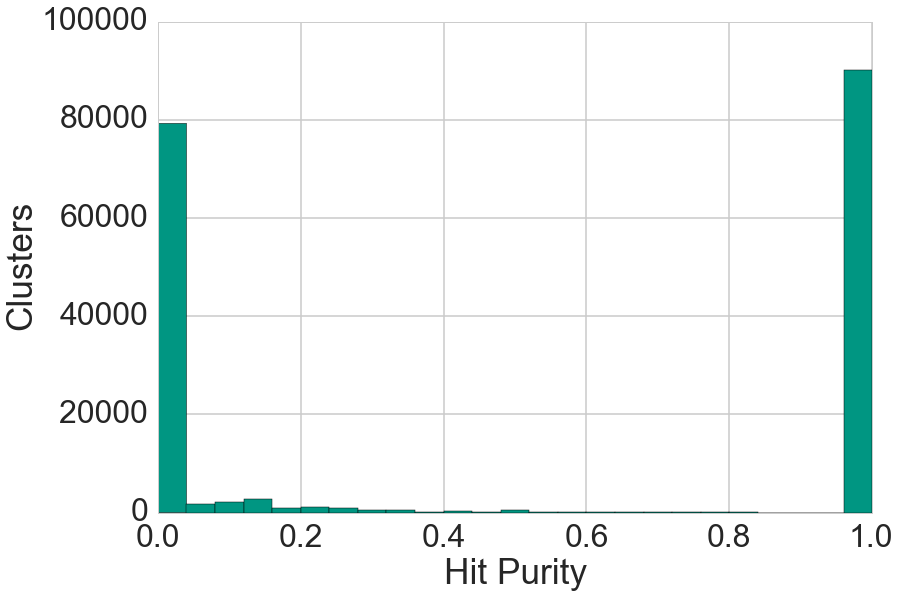
\includegraphics[width=0.7\linewidth]{figures/workflow/cluster_purity.png}
  \caption{Histogram of the hit purities (ratio between signal hits to all hits in a cluster) of the found clusters by the clusterizer as part of the local track finder algorithm. As the clusters are either purely signal or purely background, they can be kept or thrown away as whole objects.}
  \label{fig-cluster-hit-purity}
\end{figure}

In every event, each formed cluster is passed to the chosen filter with the chosen filter parameters to decide whether to use the hits in this clusters for track finding or not. This filter can return every number as a result including the C++ std::nan, which is used as the value for indicating that the cluster should not be used further for track finding as it is marked as background by the filter.

The filter design is very general and leaves the possibility open to compare many different filters. For the background filter as well as for many other used filter in the CDC tracking, five filters are implemented which can be selected by using module parameters. These filters are:

\begin{description}
  \item[BaseFilter] is a filter that neglects every item. It is the parent base object for every other filter and is rarely used in production.
  \item[AllFilter] is the counterpart of the BaseFilter and accepts all items. It can be used for testing purposes to make a filter fully transparent.
  \item[SimpleFilter] is a filter based on self-implemented cuts. The variables to cut depend on the planned usage of the filter and need to be implemented by the user.
  \item[TMVAFilter] is based on a trained boosted decision tree. It passes the variables defined in a so called VarSet to the BDT and returns a result between 0 and 1. If the result is lower than a certain cut definable on runtime, the TMVAFilter returns std::nan otherwise the result of the BDT. The variables can be freely defined by the user. In most of the cases the separating force of a well-trained TMVAFilter exceeds the one of a simple filter.
  \item[RecordingFilter] returns only a single constant defined on runtime independent on the input and can therefore not directly be called a filter. Instead, its purpose is to write the same variables as the TMVAFilter uses together with a truth information of every incoming item into a ROOT \texttt{TNTuple}. The output file with this \texttt{TNTuple} can later be used to train a BDT to categorize according to the truth information. This filter can of course only be used on simulated data.
  \item[MCFilter] filters the items according to the truth information compiled with the MC information that is also used in the recording filter.
\end{description}

As an example for the mentioned VarSet, the variables for distinguishing the background clusters from the signal clusters is described in table~\ref{tab-varset-cluster}. The truth information used for the BDT training is also described there. It is not always obvious why the described variables can help to separate between background and signal cluster. This is why one typical signal and one background cluster is shown in figure~\ref{fig-cluster-versus}. As can be seen in the figure, background clusters have a different shape as signal clusters. Particles creating signal hits pass almost straight through the wires leaving behind a defined long-shaped trace of hits whereas background hits get created in a single spot forming more circular-shaped clusters (if they have more than one hit at all). This shape-information is used in the number of neighbors as well as in the averaged distance to the superlayer center. The latter is zero for most of the signal clusters as the particles go through the whole superlayer whereas background hits do not span the whole section. As the background clusters are made of hits coming from stochastically distributed processes, the parameters of the hits like time information (which gets transformed to the drift length) or deposited energy (which is encoded in the ADC count) are probably randomly distributed. This is why the first two momenta of the distributions (mean and variance) are also taken into account.

\begin{figure}
  \centering
  \begin{minipage}{0.58\linewidth}
    \centering
    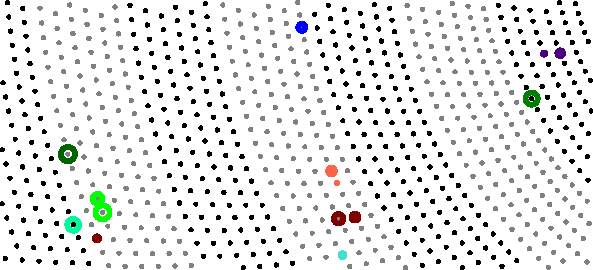
\includegraphics[scale=0.8]{figures/workflow/cluster_display_background.pdf}
  \end{minipage}
  \begin{minipage}{0.4\linewidth}
    \centering
    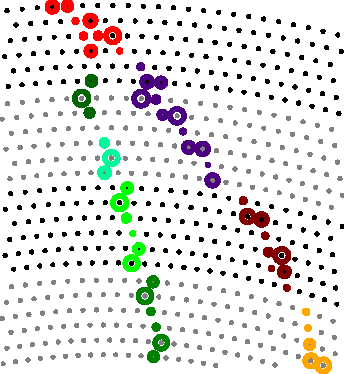
\includegraphics[scale=0.8]{figures/workflow/cluster_display_signal.pdf}
  \end{minipage}
  \caption{Detailed view of a full event display (cf. figure \ref{fig-} in chapter~\ref{chapter-theory}) with found clusters colored differently for better visualization. The left subfigure shows background clusters, whereas the right one shows clusters with hits from simulated signal particles. The differences in the described variables like shape, number or distance can be seen.}
  \label{fig-cluster-versus}
\end{figure}


\begin{table}
  \centering
  \begin{tabular}{p{0.35\linewidth}p{0.6\linewidth}} \toprule
   Variable Name & Description \\ \midrule
   \verb+is_stereo+ & Boolean variable if the cluster is in a stereo superlayer or not. Has no separating force by itself but only in combination with other variables. \\ \midrule 
   \verb+superlayer_id+ & The index of the superlayer counted from the most inner superlayer outwards. As the \verb+is_stereo+ variable, is should is used in combination with other variables.\\ \midrule 
   
   \verb+size+ & The number of hits combined to a cluster. This variable by itself has the best separation power among all variables, as background hits occur most likely as disconnected hits whereas signal hits are connected by the track they form.  \\ \midrule 
   
   \verb+total_number_of_neighbors+ & \multirow{2}{*}[-1.5pt]{\begin{minipage}{\linewidth} The number of neighbors for on hit is the count of hits in the direct surrounding of a wire hit and can therefore be at most six (as can be seen in figure~\ref{fig-sense-wires} in chapter~\ref{chapter-ex}). The sum of all neighborhood numbers for all hits in the cluster and the total number divided by the number of wire hits are used. \end{minipage}} \\[5ex] \cmidrule{1-1}
   \verb+mean_number_of_neighbors+ & \\[5ex] \midrule 
   
   \verb+total_drift_length+ & \multirow{3}{*}[-1.5pt]{\begin{minipage}{\linewidth} The drift length is a function of the measured time delta between the collision and the moment the drifting electrons touch the sense wires. The sum over all hits in a cluster, the averaged drift length and the variance is used. \end{minipage}} \\[1ex] \cmidrule{1-1}
   \verb+mean_drift_length+ & \\[1ex] \cmidrule{1-1}
   \verb+variance_drift_length+ & \\[1ex] \midrule 
   
   \verb+total_inner_distance+ & \multirow{3}{*}[-1.5pt]{\begin{minipage}{\linewidth} The inner distance is the geometrical difference between the wire position in the $r$--$\phi$ plane and the interaction point. For stereo hits, the position for $z = 0$ is chosen. \end{minipage}} \\[1ex] \cmidrule{1-1}
   \verb+mean_inner_distance+ & \\[1ex] \midrule
   \verb+distance_to_+ \verb+superlayer_center+ & Instead of calculating the distance to the interaction point, the averaged radial distance from the wire hits to the radius of the center of the superlayer the cluster lays in is calculated. \\ \midrule 
   
   \verb+total_adc_count+ & \multirow{3}{*}[-1pt]{\begin{minipage}{\linewidth} Together with the time delta of the incoming drifting electrons each sense wire measures also the number of electrons that were ionized in the drift cells. The ADC count is the digitized value of this number. \end{minipage}} \\ \cmidrule{1-1}
   \verb+mean_adc_count+ & \\ \cmidrule{1-1}
   \verb+variance_adc_count+ & \\ \midrule
   \verb+truth+ & A cluster is counted as signal if more than 80 \% of the contained hits belong to a simulated MC particle (and not to background). As the number of hits in one cluster is mostly very small, this implies that all hits must be from a signal track for most of the cases. \\ \bottomrule
  \end{tabular}

  \caption{The variables used for the classifier to separate background from signal clusters (and hits). Additional information on some of the variables can be found in the text.}
  \label{tab-varset-cluster}
\end{table}

After the recording and the training procedure (which is handled by Python scripts) the TMVAFilter with the mentioned VarSet can be used. Figure~\ref{fig-result-background-hit-finder} shows the ROC curve (left side) and the distribution of the BDT result for the training and the testing set of clusters. As can be seen, the BDT has a very good separation power between background and signal clusters. As the output distributions for testing and training data set is very similar, there is also no overtraining visible.

\begin{figure}
  \centering
  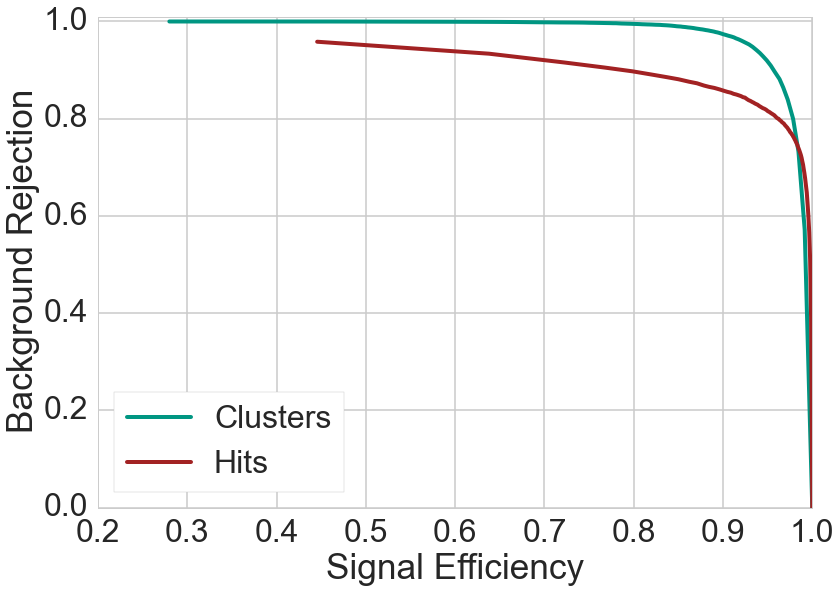
\includegraphics[width=0.48\linewidth]{figures/workflow/background_hit_finder_roc.png}
  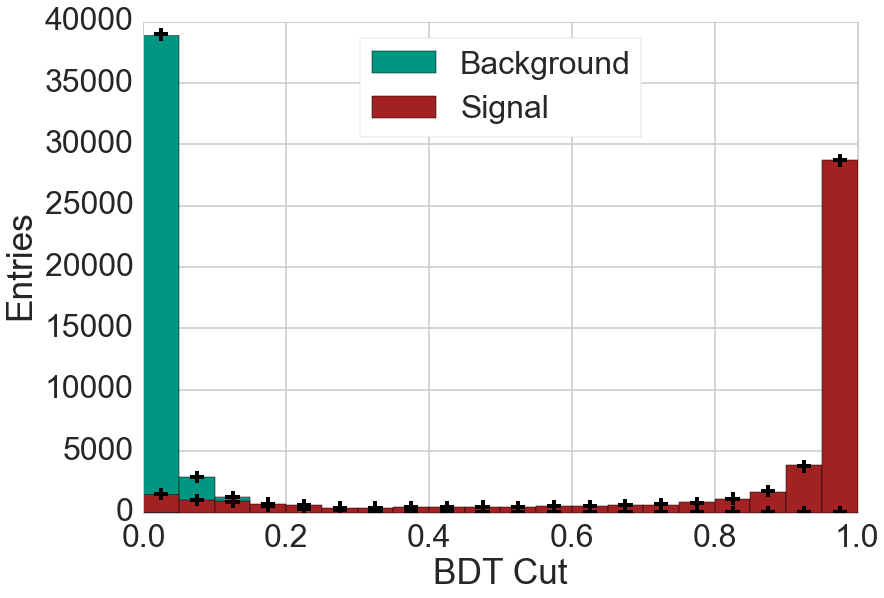
\includegraphics[width=0.48\linewidth]{figures/workflow/background_hit_finder_overtraining.png}
  \caption{The left plot shows the background rejection over the signal efficiency (so-called ROC curve) for the trained BDT to distinguish between signal and background clusters. Also shown is the ROC curve recalculated using the hits in each cluster. As the number of hits in each cluster is not constant, the two curves differ. The right histogram describes the distribution of the output variable of the BDT for signal and background clusters in the testing (cross markers) and the training (bars) data set. No overtraining is visible as the distributions match perfectly well.}
  \label{fig-result-background-hit-finder}
\end{figure}

By applying a cut on the BDT output the background hits can be marked and do net get used in the following tracking routines. How this cut is chosen depends on the desired optimization. A lower cut can include many background hits but does not throw away signal hits keeping the fake rate as well as the hit efficiency high. A harsher cut however can increase the finding efficiency as the combinatorics are reduced and the probability to collect background hits is reduced. Figure~\ref{fig-result-background-hit-finder2} shows the figures of merit of the axial Legendre track finder alone with different cuts on the BDT output. Especially the fake rate can be strongly reduced by using the background hit finder. Figure~\ref{fig-hits-numbers} shows the number of signal/background hits and clusters with different cut values. As the number of signal clusters/hits stays equal but the number of background clusters/hit is reduced with higher cut values, the combinatorics are reduced as well. This can be seen in figure~\ref{fig-performance-clusters}, where the computation time of the local track finder algorithm (which is in particular sensitive to the combinatorics) is shown.

\begin{figure}
  \centering
  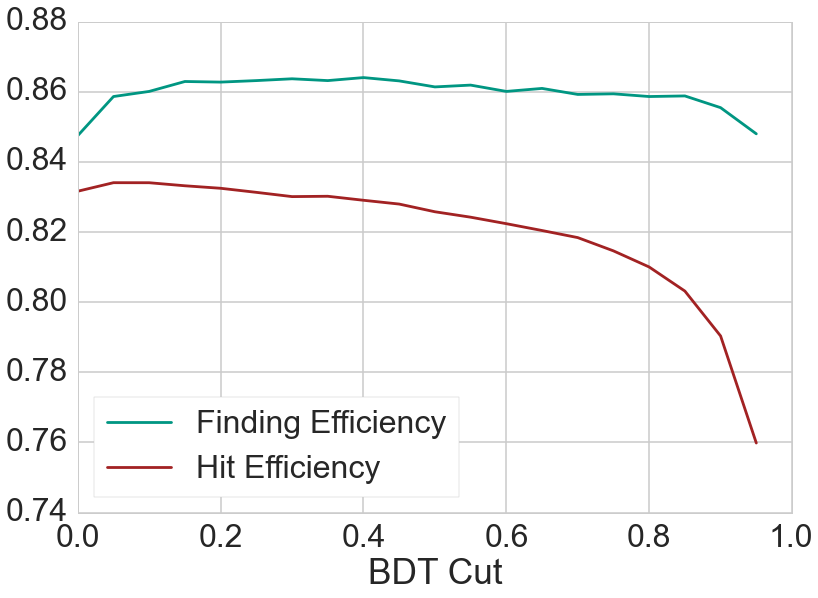
\includegraphics[width=0.48\linewidth]{figures/workflow/background_hit_finder_efficiency.png}
  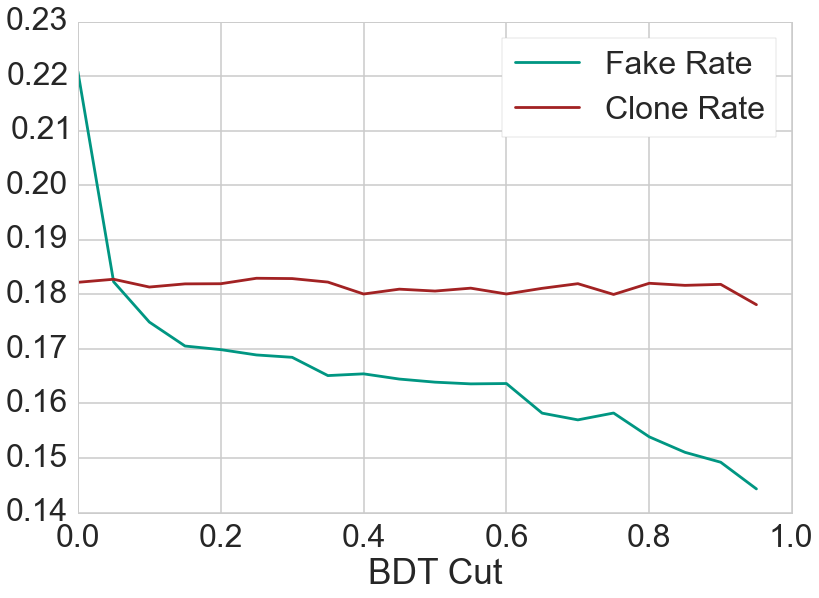
\includegraphics[width=0.48\linewidth]{figures/workflow/background_hit_finder_rate.png}
  \caption{Figures of merit of the Legendre track finder (without combination with the automaton track finder and without final track quality corrections) for different cut values on the background hit finder BDT. With the background hit finder, the rate of fakes could be reduced drastically. The finding efficiency and the clone rate stay almost the same. When the cut on the BDT output is to hard, the hit efficiency is decreased.}
  \label{fig-result-background-hit-finder2}
\end{figure}

\begin{figure}
  \centering
  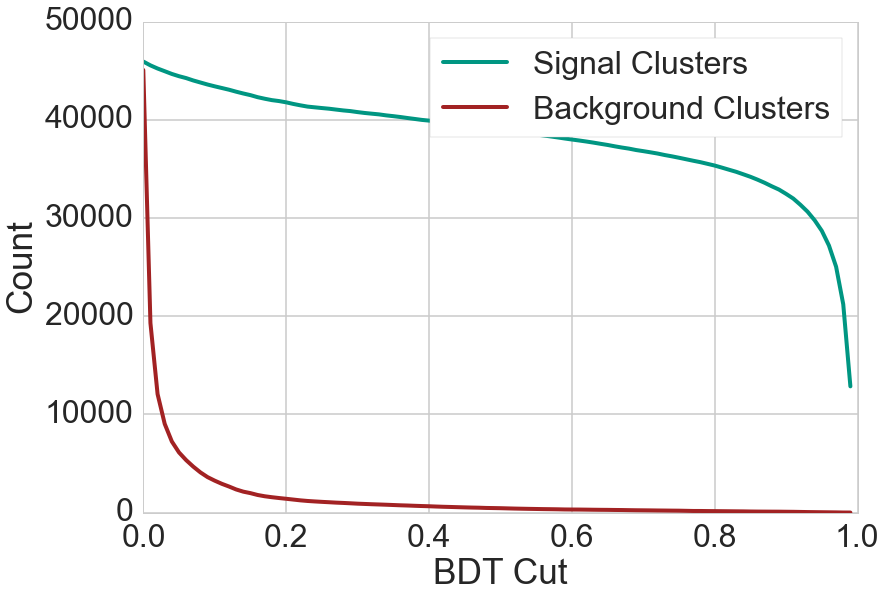
\includegraphics[width=0.48\linewidth]{figures/workflow/number_of_clusters.png}
  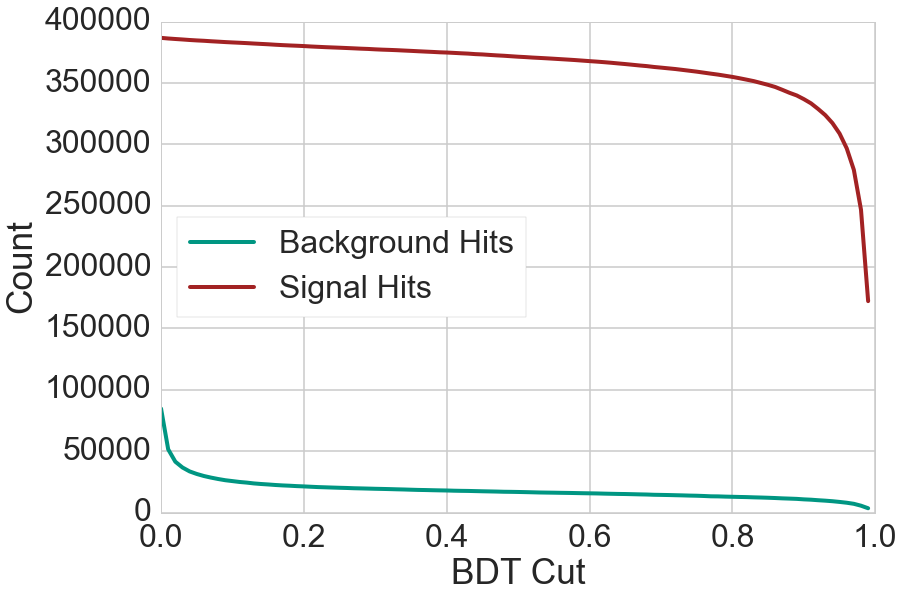
\includegraphics[width=0.48\linewidth]{figures/workflow/number_of_hits.png}
  \caption{Number of signal/background clusters/hits after a cut on the BDT output. The number of signal hits stays more or less the same for the lower cut value region whereas the number of background hits decreases.}
  \label{fig-hits-numbers}
\end{figure}

\begin{figure}
  \centering
  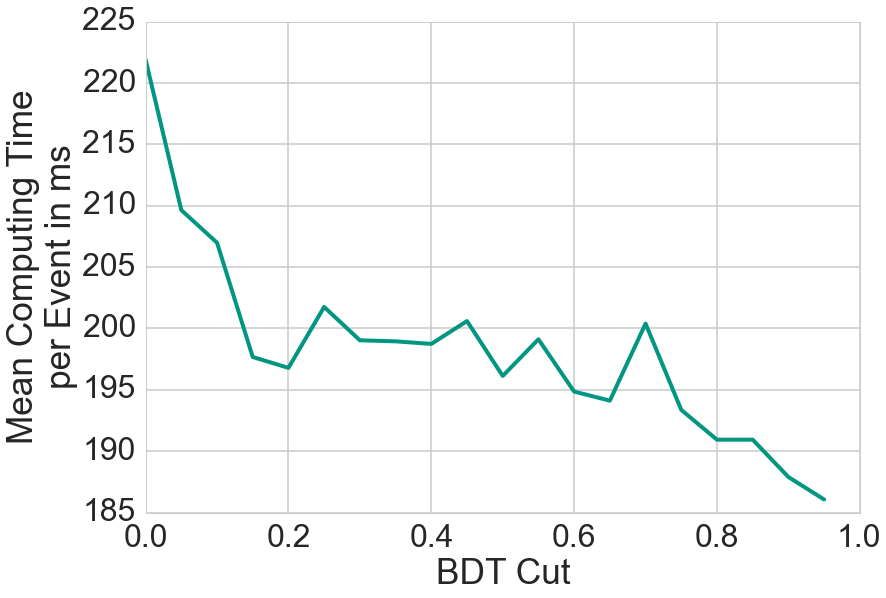
\includegraphics[width=0.6\linewidth]{figures/workflow/background_hit_finder_performance.png}
  \caption{Averaged computing time per event of the two track finder algorithms (local and global) in sum with the already implemented changes as described in the following sections for different cut values on the BDT output. Except for statistical fluctuations, the computing time decreases with harder cut, as the number of hits gets smaller.}
  \label{fig-performance-clusters}
\end{figure}

\todo{describe axial or not?}
% \section{Improvements on the Axial Legendre Track Finder}
% Is already very good and advanced. 

% \subsection{The class \texttt{QuadTreeProcessorTemplate}}
% \subsection{Postprocessing after the track finding}
% \subsection{Results}
% Timing

\section{Improvements on the Stereo Legendre Hit Finder} \label{section-stereo}

The previous implementation of the stereo hit finder yielded good finding and hit efficiencies with an acceptable fake and clone rate. However, the module was partly built with legacy code and had a very bad computing performance as the processing time of the stereo finder was about 20 times higher than the axial finder. Instead of refactoring the module, it was rebuilt from scratch in this thesis using the common code basis for all track finder algorithms in the CDC and the same quad tree structure as the axial hit finder. Additionally, a refined stereo position calculation was implemented using the already provided methods from the framework and a second coordinate in the quad tree structure was introduced. Before, the stereo hit finder used only the $\lambda$ angle for a histogramming method whereas in the new module the the slope in the $s$--$z$-plane and $z_0$ are used as described in chapter~\ref{chapter-theory}. Because of an introduced caching method, the computation could be speed up by a factor of approximately 100. The algorithm is described in the next paragraph whereas the results in comparison to the old implementation are shown after that.

\subsection{Implemented algorithm}

The stereo hit finding algorithm consists of three stages, which are repeated for every found axial track. In between the iterations for every track, the found hits are marked to not use them twice. The steps are in detail:
\begin{zlist}
  \item \textit{Fill a vector of hits and pass them to the quad tree.} All non-used stereo hits from the wire hit topology (except background hits) are used to create a vector of reconstructed hits. These hits have a cached travel distance $s$ and a $z$ position, that is calculated using the track. It is chosen in such a way, that the trajectory in the $r$--$\phi$-plane touches the drift circle of the wire hit perfectly. As there are inherently two possible orientations of the hit -- left or right -- there are two items in the vector for each wire hit. A check if the travel distance is negative (which happens for hits laying on the other side of the CDC than the track) and if the reconstructed $z$ value is outside of the CDC boundaries is applied. 
  \item \textit{Quad tree search for the best candidate.} The $\tan \lambda$ and the $z_0$ values of the passed right--left-items in the vector are used in a quad tree search. For this, a line in the $s$--$z$-space is constructed with the slope $\tan \lambda$ going through $(0, z_0)$. An item belongs to a quad tree bin if and only if this line goes through the bin borders exactly twice (which can easily be checked using the mean value theorem). As only one single axial track is used for reference at a time, only the highest bin in the quad tree search is used. If both the right and left hypothesis of a hit are in the resulting bin, the one orientation laying more near to the trajectory is used.
  \item \textit{Add the found hits to the axial track and clear the quad tree.} After the search is finished, the found stereo hits are added to the axial hits and the whole track hits are sorted correctly. For this, a line fit is performed to extract the $z$-information of the trajectory. In the end, the quad tree is cleared and prepared for the next track or event.
\end{zlist}

Both quad tree algorithm implementations currently available in the framework are used in the module and can be switched easily by module parameters. As they both use the same principles, only the results of one implementation are shown. Additionally, as base items for the vector passed to the quad tree not only stereo wire hits but also stereo segments coming from the local track finder can be used. Instead of checking if the line in the $s$--$z$-plane intersects with the quad tree bin for a single hit, all hits in the segment are checked for. If more than 70 \% of the hits in a segment intersect with a quad tree bin, the whole segment is counted in in this bin with the number of intersecting hits as a weight. Using segments instead of hits has some benefits: as the hit purity of the segments is rather high, adding whole segments instead of single hits can improve the hit efficiency and purity of the stereo tracks. Also, as the number of segments is much smaller than the number of hits, the combinatorics in the quad tree search is reduced resulting in a smaller quad tree level and a smaller computing time. The drawback, however, is that single wrong or wrongly reconstructed\footnote{As the $z$-position reconstruction depends heavily on the trajectory parameters in the $r$--$\phi$-plane, the calculation can give wrong results when these parameters are off because of energy loss or low hit purity of the axial hist.} hits can influence the segment quite much. The problem is, that if a whole segment is lost because of a few wrong hits, the hit efficiency is reduced.

\subsection{Results}

The two operation modes in the new stereo hit finder module (with bare wire hits or with segments) can be compared to the old stereo hit finder implementation and also with the reference implementation trasan from Belle. The figures of merit and the computation time per event are shown in table~\ref{tab-stereo-results} together with the finding and hit efficiency as a function of $p_T$ in figure~\ref{fig-stereo-results}. 

\begin{table}
  \todo{Results stereo.}
  \caption{}
  \label{tab-stereo-results}
\end{table}

\begin{figure}
  \todo{Results stereo.}
  \caption{}
  \label{fig-stereo-results}
\end{figure}

As can be seen, the figures of merit are enhanced by the newly written module and are now comparable or better than the reference implementation. This is mainly because of the additional coordinate in the quad tree which handles track not coming from the interaction point. The computing time is much smaller which is mainly because of caching and optimized calculation procedures, e.g.\ by changing the coordinates in the Legendre space from $\lambda$ which needed heavy trigonometrical calculations to the much easier to calculate $s$--$z$-slope.

\section{The \texttt{SegmentTrackCombinerModule}} \label{section-combiner}
\subsection{Principle of the Segment Track Combiner}
+ Task
\subsection{Used Filters}
\subsection{Results}

\section{The \texttt{Track\-Quality\-Asserter\-CDC\-Module} and the \texttt{Track\-Quality\-Tools}}  \label{section-quality}

The common code basis in the CDC track finding package make it possible to include common correction tools for the resulting tracks into the software framework. The \texttt{Track\-Quality\-Tools} singleton offers functions for applying typical corrections on the track candidates like removing of hits or normalizing the trajectory information to a defined format (e.g.\ the start point of the circular trajectory should lay on the position of the first hit). The different implemented methods are described later.

These tools can be used in the track finder modules directly (instead of implementing the same algorithms again), but are also used standalone (with the module \texttt{Track\-Quality\-Asserter\-CDC\-Module}) after the whole track finding procedure. The reason is not only to reduce the number of wrong hits per track and the fake rate, but also to prepare the tracks for the next step, the track fitting. The fitting algorithm needs a defined format for the trajectory seed parameters (the position seed must lay near the first hit in the track and the momentum seed must be defined at this point). Additionally, the fitting algorithm as it is currently implemented in the framework is very sensible to discrepancies in the track candidates like long segments of missing hits or wrongly added hits because of decay-in-flight particles or high energy loss. The fit can get biased into a wrong direction in the first iteration leading to an increased number of steps and because of more needed material lookups a higher computing time. As the maximal number of iteration per track is limited to improve performance, the fit can fail completely reducing the finding efficiency when taking into account only fitted tracks to about 60 \% (compared to the values of about 90 \% before the fit). To increase the number of successful fits, the tracks can be edited to be suited for fitting including the clipping of hits which reduces the hit efficiency. As only the tracking parameters at the front of the track are important for physics analysis, cutting away parts of the track does not harm the fit resolution directly. The hits however can be used in $\mathrm d E/\mathrm d x$ analysis for particle identification and it may be a good idea to keep the relation to the track and readd them to the fitted results to increase the hit efficiency again. 

Another important step is the removal of axial only tracks which can not be fitted by the currently implemented track fitting procedures as there is no direct $z$ information present in the tracks.\footnote{Tracks without stereo hits have nevertheless a $z$ information in them as the energy loss depends in the travel length in the material which in turn is related to the $\theta$ angle of the track. \cite{martin}} As most of these tracks have no stereo hits because the energy is too low to reach into the first stereo superlayer and not because the track finder algorithms have not found the hits there is no possibility to add stereo information to the tracks in the CDC only. For a different approach -- combining the CDC track candidates with the VXD results -- are shown in section~\ref{section-outlook}.

After running the \texttt{Track\-Quality\-Asserter\-CDC} module before fitting the finding efficiency when only taking into account fitted tracks could be increased but does not reach the finding efficiency before the fit -- so the fitting rate is not 100 \% still. The finding and hit efficiency together with the other figures of merit are shown in table~\ref{tab-results-after-fitting} before and after the fit with and without the quality module. Also, the computing time of the fitting module could be reduced from \todo{numbers}. Once the external fitting package is improved to handle these challenging cases also, some of the corrections can be turned off by changing the steering file parameters of the module.

\begin{table}
  \todo{Results after fitting.}
  \caption{}
  \label{tab-results-after-fitting}
\end{table}

Some of the methods implemented in the \texttt{TrackQualityTools} are described with full details in the following:
\begin{description}
 \item[\texttt{normalizeHitsAndResetTrajectory}] To have a defined starting point in each of the modules and especially for the fitting routines, the trajectory is shifted to start near the first track hit. This hit is determined to be the most inner hit of the track and has an arc length of zero. All other hits have positive arc lengths and are sorted according tho these values. The trajectory for curling tracks is reversed if the number of hits on the ingoing arm is grater than on the outgoing one.
 \item[\texttt{removeHitsAfterLayerBreak} and \texttt{removeArcLength2DHoles}]  As the fitting procedure can not handle tracks with large segments of not found hits very well it is feasible to have routines which cut tracks before those holes. This can be done either by looking on the arc length or the geometrical distance between successive hits in the tracks. An additional method can cope with multiple ``breaks'' in the track and chooses the longest coherent track part.
 \item[\texttt{removeHitsOnTheWrongSide}] The Legendre track finding algorithm has some issues with non-curling back-to-back tracks or at least hits. The problem is described in figure~\ref{fig-b2btrack}. For non-curling tracks these added hits can easily be spotted by looking onto the arc length values which is negative for these hits.
 \item[\texttt{splitSecondHalfOfTrack}] As the reference implementation trasan, which was used successfully in combination with the fitting algorithms currently implemented, splits every curling track on the apogee point, this feature is also implemented in the track quality tools.
\end{description}
In addition, there are methods to remove tracks with a small number of hits or which are localized to a single super layer and other methods which are not described here.

\section{Further Approaches} \label{section-outlook}
\subsection{Quad tree search with segments}
Benefits: Purity high, more or less no reassignment needed. RL-information already present, lower combinatorics = more then one axis possible?

More than one possibility to do that: axial + stereo or only stereo or only axial, when should a segment belong to this legendre bin?

\subsection{VXD-CDC-Merger before fitting}
Benefits: Possible better efficiency (no loss because of fit). Faster, less fakes, better finding efficiency (because a track is kept which would be maybe deleted by a quality tool)

Ho to do it: BDT with trained variables. First results.
  \chapter{Analysis of the implemented Track Finder}
\section{Comparison of the two track finder}
\section{Tracking efficiency with different input parameters}
\subsection{Tracking efficiency with different particle and background types}
\subsection{The TMVA filters}
  \newcommand{\dedx}{$\mathrm d E / \mathrm d x$ }
\chapter{Momentum estimation of slow pions with the ADC in the VXD} \label{chapter-vxd}

When looking onto the typical momentum distribution of particles flying through the tracking detectors as show in figure \ref{fig-particles-momentum}, it is clear that there is a significant amount of so called slow pions with momenta in the order of $\unit[100]{MeV}$. Slow pions play an important role for the physics analysis planned for the Belle II experiment as they are extensively used in flavor tagging decays (e.g. $\PDstar^\pm \to \PDzero \Ppipm$). Measuring the momentum of these particles leads to a better resolution in the momenta of the parent particles $\PDzero$ and $\PDstar$ which is used in separating continuous background from signal events. These slow pions get produced near the interaction point and because of their small momentum and therefore high curvature and their huge energy losses they can not be detected in the CDC tracking detector. This means they can only be measured in the VXD. Because of the small radius of the VXD and the resulting small number of independent measurement points, the momentum resolution is very poor as it can be seen in the Glückstern formula
\begin{align*}
 \frac{\sigma_{p_T}}{p_T} = \sqrt{\frac{720}{N + 4}} \sigma_x \frac{p_T \text{[GeV]}}{0.3 q B \text{[T]} L^2}
\end{align*}
where $L$ is the length of the track in the detector and $N$ is the number of measurement points. Decreasing the magnetic field $B$ would decrease the curvature of the low momentum pions and would therefore make them detectable in the CDC also increasing the number of measurement points. But this would also make the resolution of the high momentum particles very poor. In this thesis a different approach is chosen. Together with the measured positions for each found VXD sensor hit an independent momentum estimation based on the energy loss per travel length of the particles in this sensor is calculated and used in the trajectory fit after the track finding. These added measurements bias the fit towards the correct momentum and can therefore help to increase the momentum resolution.

\begin{figure}
 \centering
 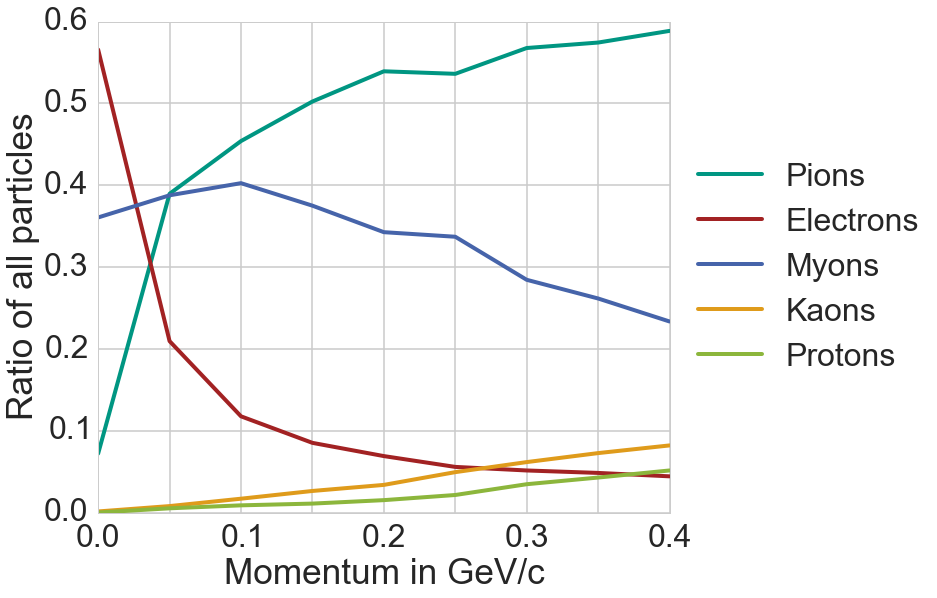
\includegraphics[width=0.8\linewidth]{figures/vxd/momentumDistribution.png}
 \caption[Momentum distribution by different particle types.]{Momentum distribution split by different particle types as generated by the simulation. As this simulation is modeled after the physical branching fractions the here shown distribution is also the expected observation in the experiment.}
 \label{fig-particles-momentum}
\end{figure}

As it was shown in previous studies~\cite{robert}, the momentum resolution compared to the result of the helix fit with the positions only can be increased by using the information from the energy loss of all hits in the track together. In the quoted paper an advanced summation was used to build a truncated mean energy loss of the slow pions which was transformed to a momentum by a predetermined formula. This momentum estimation was then compared to the one coming from the helix fit. To increase the resolution even more, the two different approaches - helix fit and ADC count - are combined in the presented algorithm.

In figure \ref{fig-dedx-over-p} the energy loss per travel length in the VXD sensors for low momentum pions is shown. How these numbers are calculated is described in the next sections. As it can be seen, the \dedx value increases with falling momentum of the particles. This relation can be also seen in the already quoted Bethe formula \ref{form-bethe} in chapter \ref{chapter-ex} which can be reduced to 
\begin{align}
 -\left \langle \dd{E}{x} \right\rangle \approx \frac{4 \pi n z^2}{m_e v^2} \left( \frac{e^2}{4 \pi \varepsilon_0} \right)^2 \ln \left( \frac{2 m_e v^2}{I} \right) \label{form-bethe-simpl}
\end{align}
for small particle energies. The equation can theoretically be used to calculate the momentum using the energy loss per travel length. But as this formula describes the averaged energy loss, it is only correct for a small number of cases. The variance in the energy loss is distributed according to a landau distribution which is described later in more detail. This deviation from the Bethe formula decreases the momentum resolution of the estimation based on the energy loss.

\begin{figure}
 \centering
 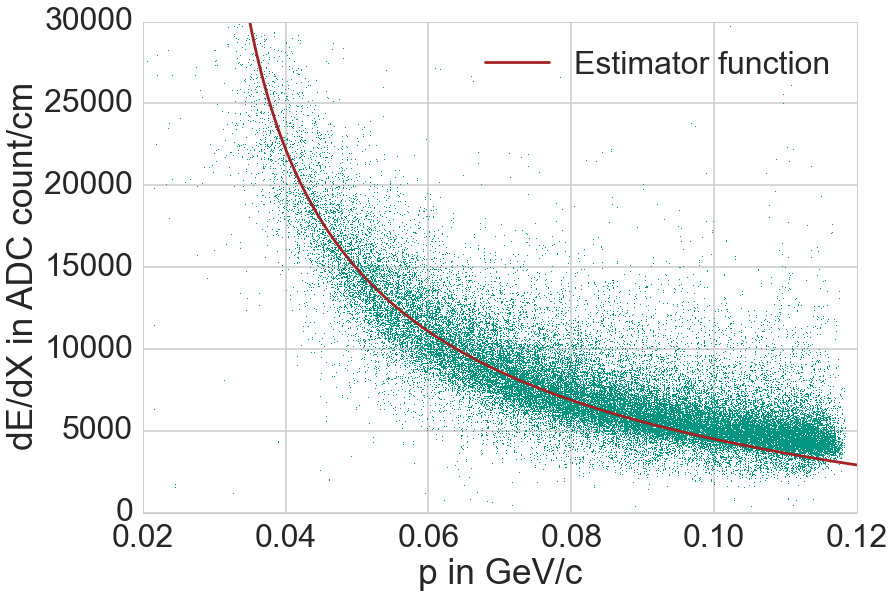
\includegraphics[width=0.8\linewidth]{figures/vxd/dedxWithEstimator.png}
 \caption[\dedx information of the VXD clusters.]{\dedx information of the VXD clusters of approximately 100000 pions in the momentum range from 50 to 120 MeV. The averaged energy loss can be described by the Bethe formula. The distribution of energy losses for a given momentum is distributed according to a landau distribution which is described later in more detail. To transform the \dedx value to a momentum the red estimator curve is used later.}
 \label{fig-dedx-over-p}
\end{figure}


\section{Prestudies on the distribution of dE/dx in the VXD}

For the following studies an event sample of slow pions in the momentum range between $\unit[50]{MeV}$ and $\unit[120]{MeV}$ is used. It is simulated using the particle gun with 10 particles per event evenly distributed among the momentum range and between the two charge modes. The sample is split into different event samples for testing and training. The standalone VXD track finder or the MC track finder for reference is used to create tracks out of the simulated VXD hits. As the finding efficiency of the standalone VXD track finder depends heavily on the momenta of the particles, the distribution of the found tracks is not flat any more as it can be seen in figure \ref{fig-vxd-finding-efficiency}. A typical event display can be seen in picture \ref{fig-vxd-event-display}.

\begin{figure}
 \centering
 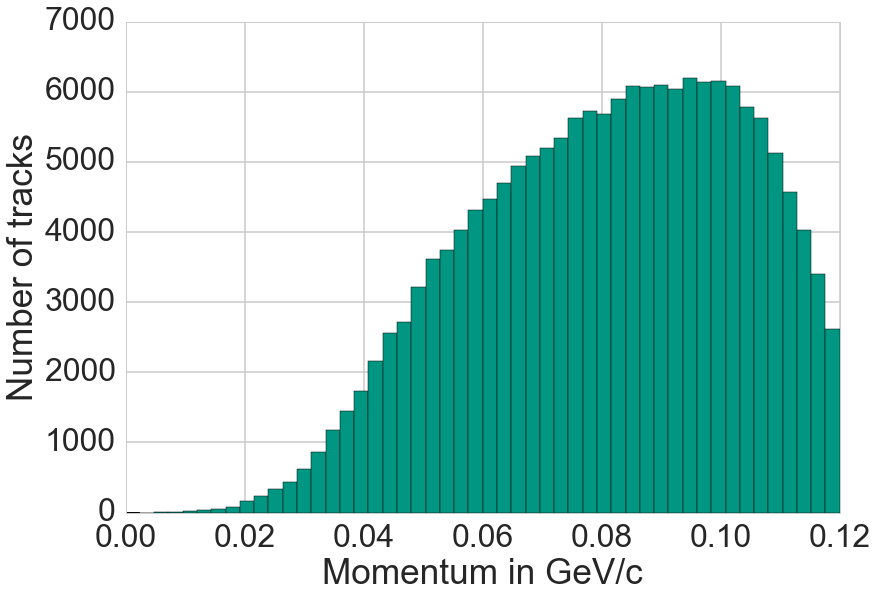
\includegraphics[width=0.48\linewidth]{figures/vxd/finding_efficiency.png}
 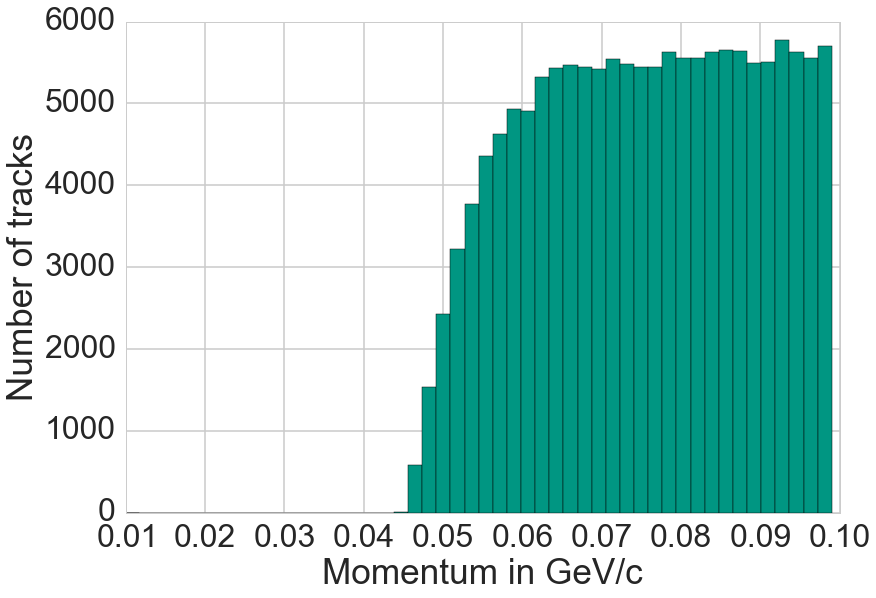
\includegraphics[width=0.48\linewidth]{figures/vxd/finding_efficiency_mc.png}
 \todo{why is there a drop?}
 \caption[Momentum distribution of the found and simulated pions.]{Momentum distribution of the simulated pions as found by the VXD track finder (left) and the MC track finder (which has the simulated truth information, right). The finding efficiency decreases with lower momenta as the number of hits in the VXD is lower for slow pions and the energy loss is stronger. The MC track finder has also not a flat distribution of momenta as it only uses those particles for tracks which have at least 3 hits in the VXD detector.}
 \label{fig-vxd-finding-efficiency}
\end{figure}

\begin{figure}
 \centering
 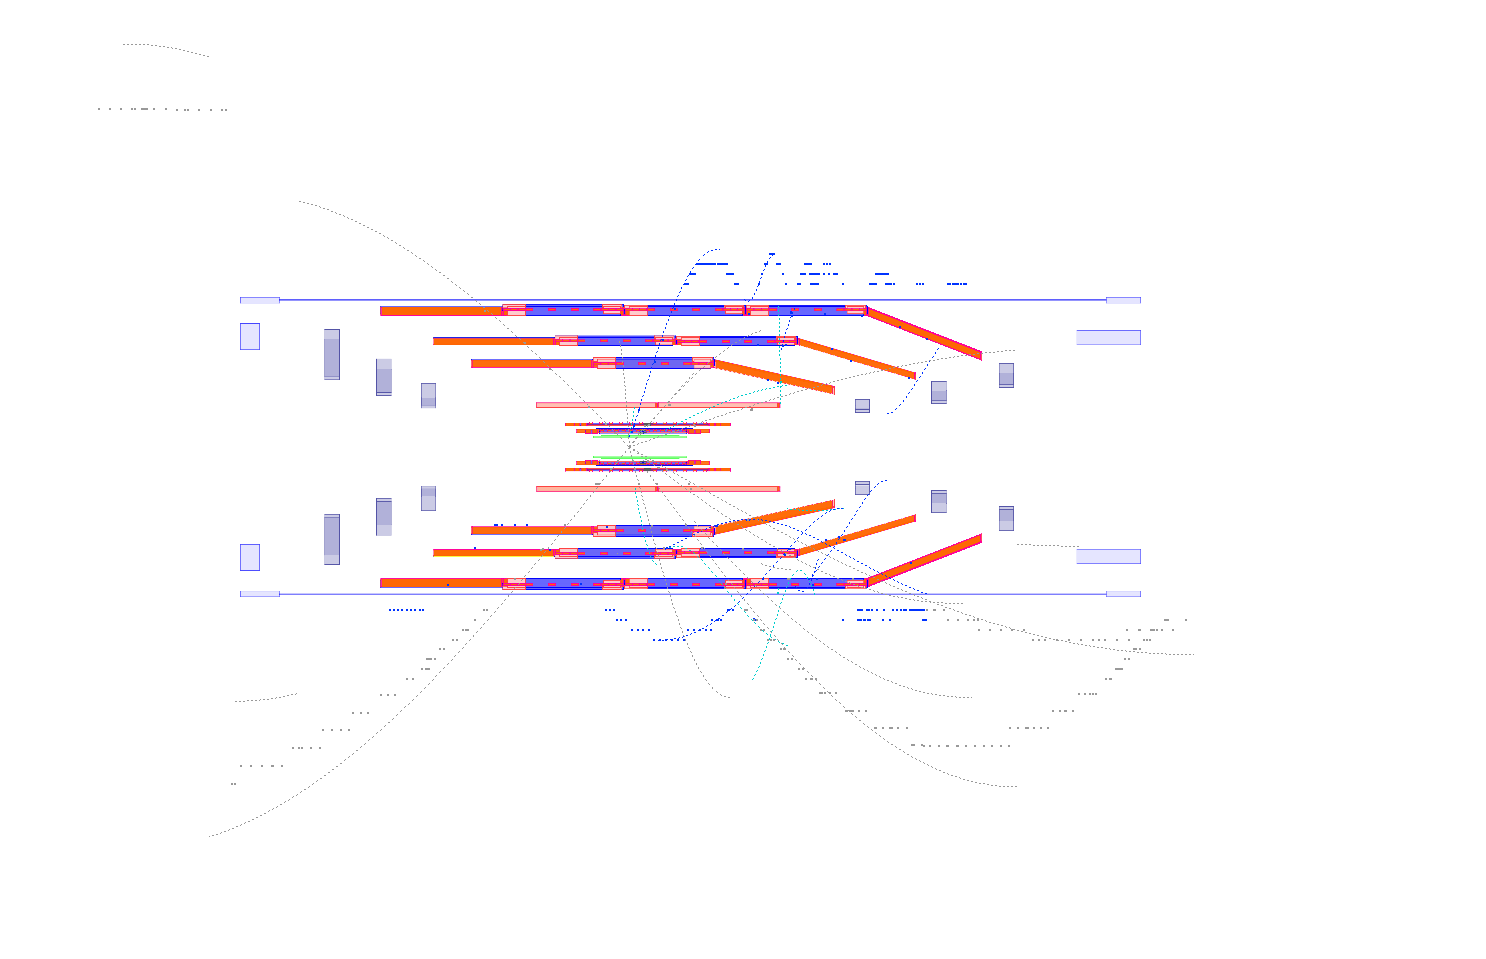
\includegraphics[width=0.8\linewidth]{figures/vxd/event_display.png}
 \caption[Typical event display of slow pions.]{Typical event display of one event used for analyzing the momentum estimation for the fitting procedure in the helix fit. The blue box depicts the inner wall of the CDC. As it can be seen, most of the particles do not reach into the drift chamber far enough and can only be detected with the VXD sensors.}
 \label{fig-vxd-event-display}
\end{figure}

Before calculating the function to transform the \dedx value to a momentum estimation and using this information in the helix fit some prestudies are performed to check for the consistency of the input data. They are shown here for reference too.

For calculating the path length used in \dedx the correct position of the hit and the sensor information is needed. This information is provided by the clusters used in the track finder. Its results can be seen in figure \ref{fig-cluster-position} where the distance to the beam pipe over the z position is shown for some SVD hits. Comparing this to the drawing of the detector in chapter \ref{chapter-ex}, a good agreement can be seen.

\begin{figure}
 \centering
 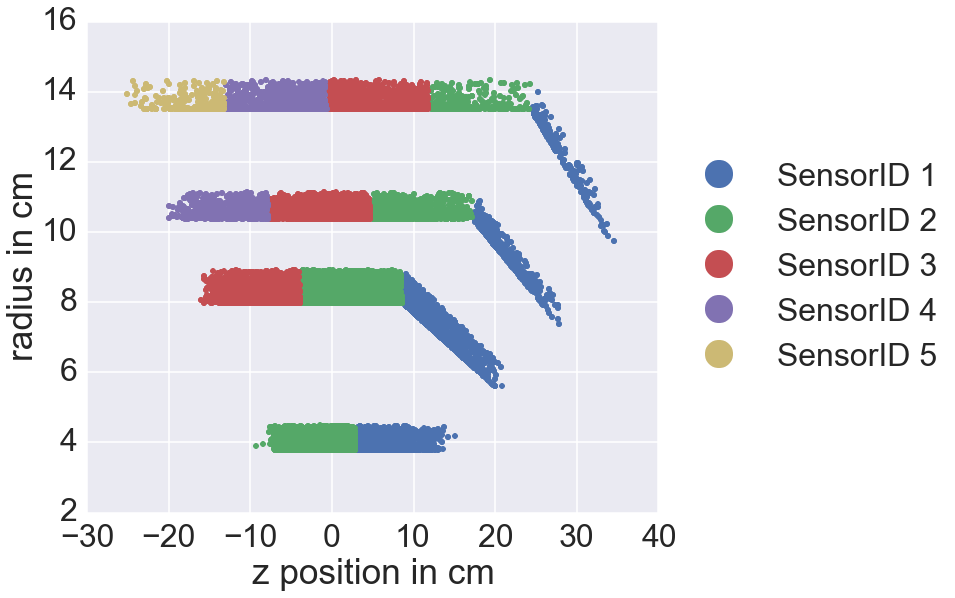
\includegraphics[width=0.8\linewidth]{figures/vxd/cluster_positions.png}
 \caption[Picture showing the simulated hit information.]{Picture showing the simulated hit information of the first 1000 clusters in the event sample. The color code separates between the sensor ID property of the clusters.}
 \label{fig-cluster-position}
\end{figure}

Instead of using the deposited charge in every sensor directly the ADC count value of every sensor is used. This ADC count comes directly from the digitalization process. It is directly proportional to the deposited energy, but this calibration coefficient has to be determined. %%%
Picture \ref{fig-adc-count} shows the \dedx value calculated with this ADC count for the two different detectors SVD and PXD. As it can be seen, the calibration coefficients for the correct deposited energy are different for the two detectors and therefore the two distributions are not superimposable. To cope with this fact the ADC counts coming from the PXD sensors get multiplied by a factor of 0.565868 which was calculated on data. The resulting distribution is shown in the right subplot of figure \ref{fig-adc-count}. This calibration is mainly done to be able to treat both hit types in the same manner later. 

\begin{figure}
  \centering
 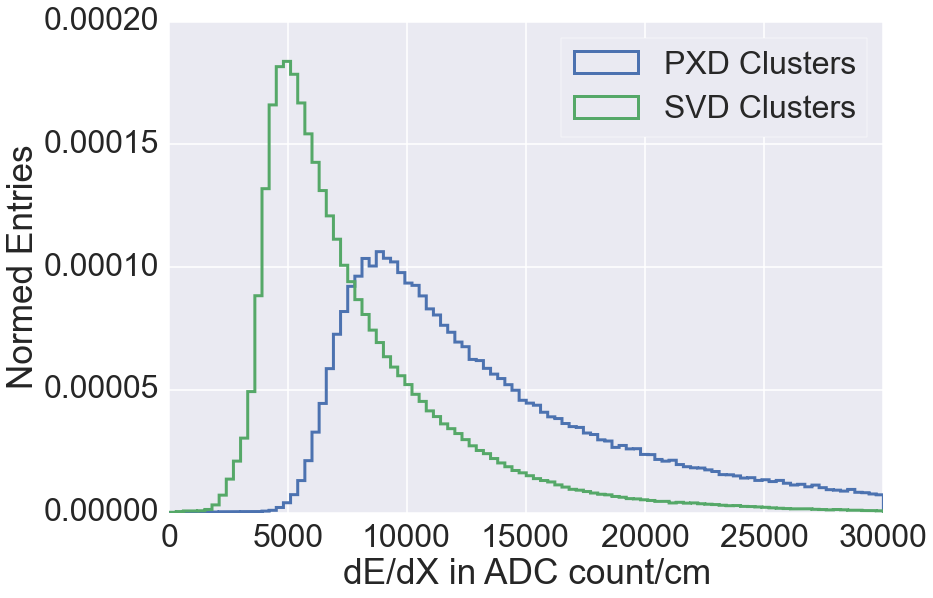
\includegraphics[width=0.48\linewidth]{figures/vxd/dEdXUncalibrated.png}
 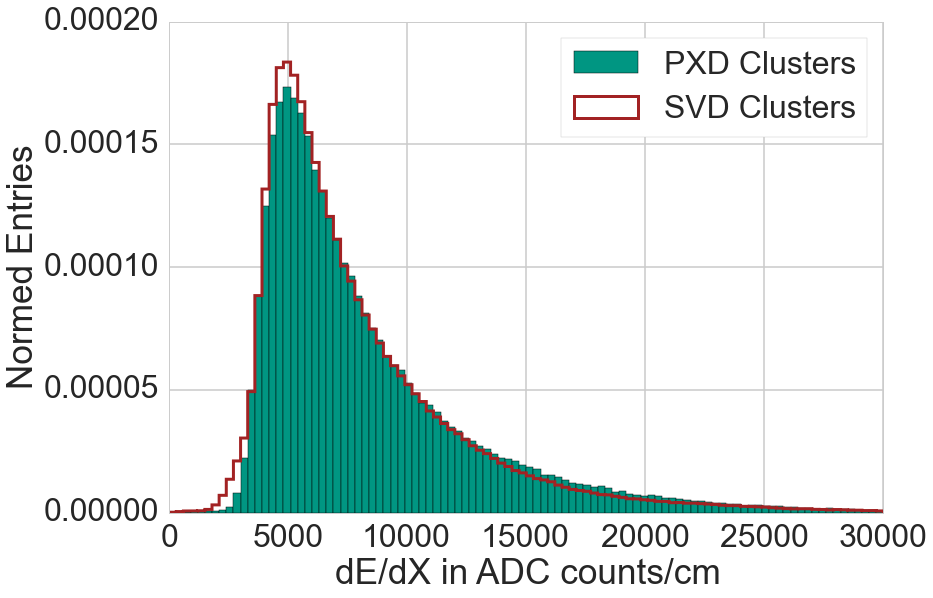
\includegraphics[width=0.48\linewidth]{figures/vxd/dEdXCalibrated.png}
 \caption[Distributions of the uncalibrated and the calibrated ADC counts.]{Distributions of the uncalibrated (left) and the calibrated (right) ADC counts of the PXD and SVD hits. Only clusters found by the VXD track finder are shown here.}
 \label{fig-adc-count}
\end{figure}

\subsection{Calculation of the path length in the clusters} \label{subsection-calc}
The \dedx value in every cluster can be calculated using the calibrated charge as described above and the length of the path the particle travels in the sensor region. There are five ways to calculate this path length. All of them are implemented in the code basis.
\begin{zlist}
 \item Using the correct (simulated) MC trajectory information of the tracks at the position of the clusters, \label{list-mc}
 \item Using the current trajectory parameters while fitting,
 \item Using the related MC trajectory at the origin,
 \item Using the trajectory parameters estimated by the track finder,
 \item Using the thickness of the cluster.
\end{zlist}

The different possibilities are ordered by their anticipated correctness. The two MC modes are only implemented for reference as they can obviously not be used in the later detector measurement. How the current trajectory parameters are deduced in the fit is described later.

Besides the last possibility, all modes rely on calculating the path length of a trajectory using their helix parameters. As the path lengths are very small, this is done without taking into account energy loss or material effects. The procedure is as follows:
\begin{zlist}
 \item Take the position of the cluster hit (the point where the trajectory enters the VXD sensor) and calculate the distance to the beam line. This is called the inner radius of the cluster.
 \item Add the sensor thickness to this radius to gain an estimation of the outer radius of the sensor.
 \item Calculate the arc length between these two radii and from this arc length the distance between the two penetration points of the helix through the sensor using trigonometrical relations.
\end{zlist}

This procedure is correct for most of the time but fails in some rare cases. Some examples are shown in figure \ref{fig-errors-in-path-length}. As it can be seen in the pictures, errors in the calculation occur mainly for particles which have their apogee\footnote{The apogee is the opposite to the perigee - the point on the helical trajectory the most far away from the interaction point} in the sensors. As the VXD sensors have only a very thin thickness the probability for such cases is very rare. Therefore these errors do not bias the momentum measurement much. Also as the calculation error can only occur in the most outer sensor touched by the particles all other sensors give correct momentum estimations. A short preliminary study shows that only about 0.4 \% of the particles are affected.

\begin{figure}
  \centering
  \raisebox{-0.5\height}{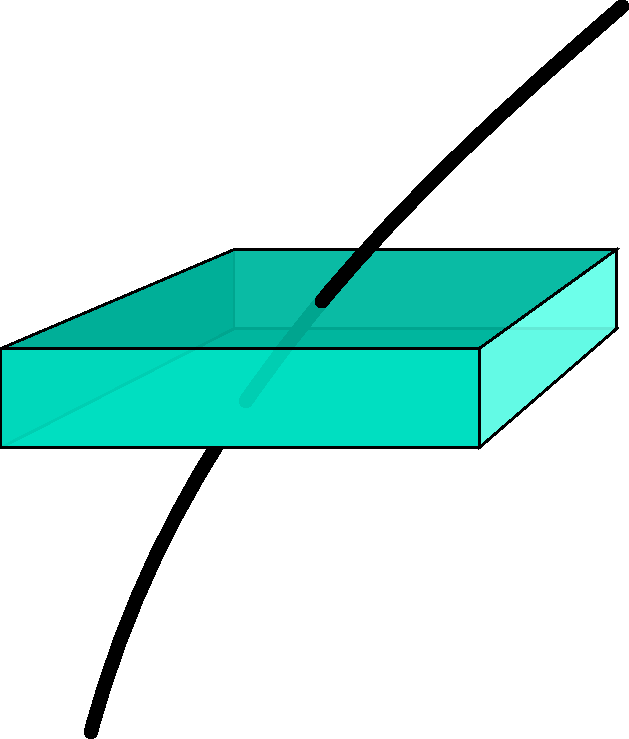
\includegraphics[scale=0.3]{figures/vxd/pathlength1.pdf}}
  \hspace*{1.5cm}
  \raisebox{-0.65\height}{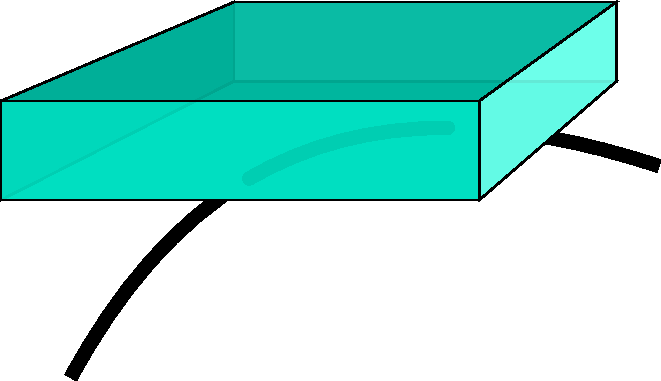
\includegraphics[scale=0.3]{figures/vxd/pathlength3.pdf}}
  \hspace*{0.5cm}
  \raisebox{-0.5\height}{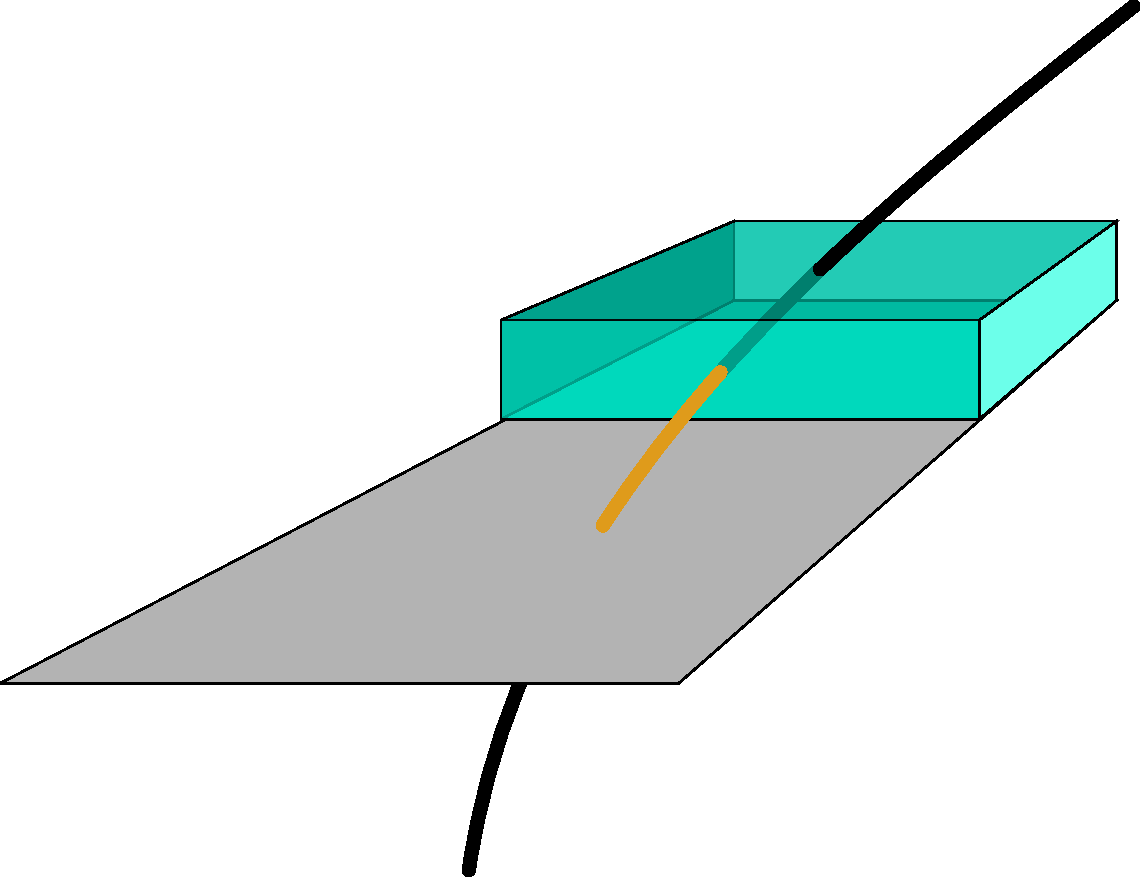
\includegraphics[scale=0.3]{figures/vxd/pathlength4b.pdf}}
  \caption[Exemplary cases of path length calculations.]{Exemplary cases of path length calculations. The algorithm fails in the second and last case. In the second case it returns the width or the length of the sensor instead. In the last case it wrongly adds the orange part of the path length to the correct one. Because of the geometrical dimensions of the sensors these two cases are very rare.}
  \label{fig-errors-in-path-length}
\end{figure}

In figure \ref{fig-pathlengths} the distribution of the path lengths from the simulated MC truth values is shown. As most of the particles go more or less straight through the sensors, there are two peaks in the distribution - one for each hit type as the two types PXD and SVD have a different thickness. Deviations from the thickness come from curling particles.

The second subplot shows the distribution of the residuum of the other three path length calculations to these reference values as a box plot. As it can be seen, the deviation to the MC hit information is most of the times below a few percent.\footnote{The box in the boxplot indicates the quartile range, whereas the big horizontal lines describes the median value. The smaller horizontal lines at the top and at the bottom show the maximum and minimum value - except for outliers.} As expected, the MC information of the track at the origin not taking into account any energy loss performs worse than the current state in the fit. What is surprising is that the track information at the origin seems to describe the path better than the current fit state. When using these values for a momentum estimation (see figure \ref{fig-result-fit2}) however, this difference is gone.

\begin{figure}
 \centering
 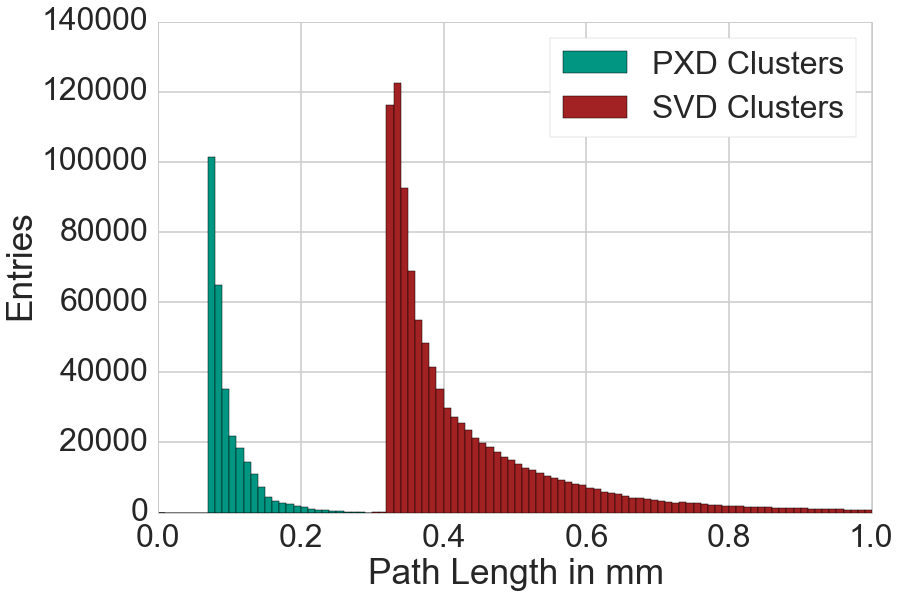
\includegraphics[width=0.47\linewidth]{figures/vxd/pathLengths.png}
 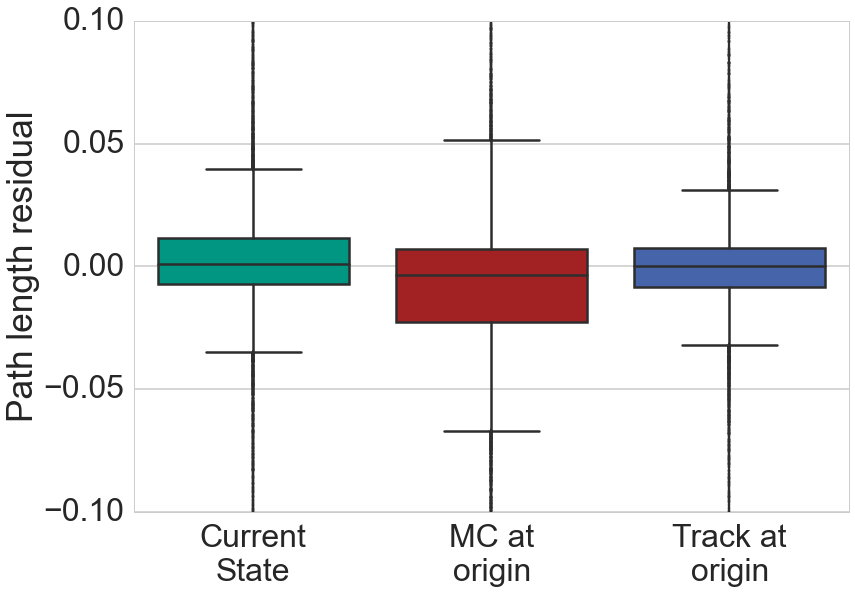
\includegraphics[width=0.47\linewidth]{figures/vxd/box_plot.png}
 \caption[Path length distribution for the two sensor types.]{The plot shows the path length distribution for the two sensor types as a result of the simulation. This distribution is used as reference in the right plot which shows the residuum distribution of the other path length calculation modes. The path length from the thickness of the cluster are not shown here as they are too far off.}
 \label{fig-pathlengths}
\end{figure}

\subsection{Transformation function from dE/dx to momentum} \label{subsection-transform}

For calculating a momentum estimation from the \dedx value the inverted function of equation \ref{form-bethe-simpl} is needed which can not be calculated analytically. Therefore a much easier model function
\begin{align}
 p(\mathrm{d}E/\mathrm{d} x) = \frac{a}{(\mathrm{d}E/\mathrm{d} x - b)^2} + c \cdot \mathrm{d}E/\mathrm{d} x + d \label{form-model}
\end{align}
with the free parameters $a, b, c$ and $d$ is fitted to the $\mathrm d E / \mathrm d x$-momentum-pairs where \dedx is calculated with path lengths from mode (\ref{list-mc}) and the momentum is taken from the MC simulation at this cluster (so including energy loss by material effects).

The free parameters can not be determined by fitting the model function to the whole dataset at once as shown for example in figure \ref{fig-dedx-over-p}. The reason is that because of the landau distributed energy loss the number of outliers is too high and causes the fit to fail. An example of the landau distribution showing the large amount of outliers deviating from the mean energy loss is shown in picture \ref{fig-landau}. This is why a reduce approach is chosen here: First the $\mathrm d E / \mathrm d x$-range is split into several small bins. In each of them the momentum distribution is build. This distribution is then fitted with a landau or a normal distribution. Mathematically, the momentum distribution in these $\mathrm d E / \mathrm d x$-bins is neither distributed according to a landau nor a normal distribution but the correct form can not be calculated analytically and these two distributions describe the data best.\footnote{The correct form of the distribution can be calculated by integrating over parts of the landau distribution folded with the inverted Bethe-equation, which is not analytically solvable.} The resulting parameters of the distributions (the mean of the normal or the location parameter of the landau distribution~\cite{landau}) are then used for fitting the model function in equation (\ref{form-model}). The whole process can be seen in figure \ref{fig-fit-bins}.

\begin{figure}
  \centering
  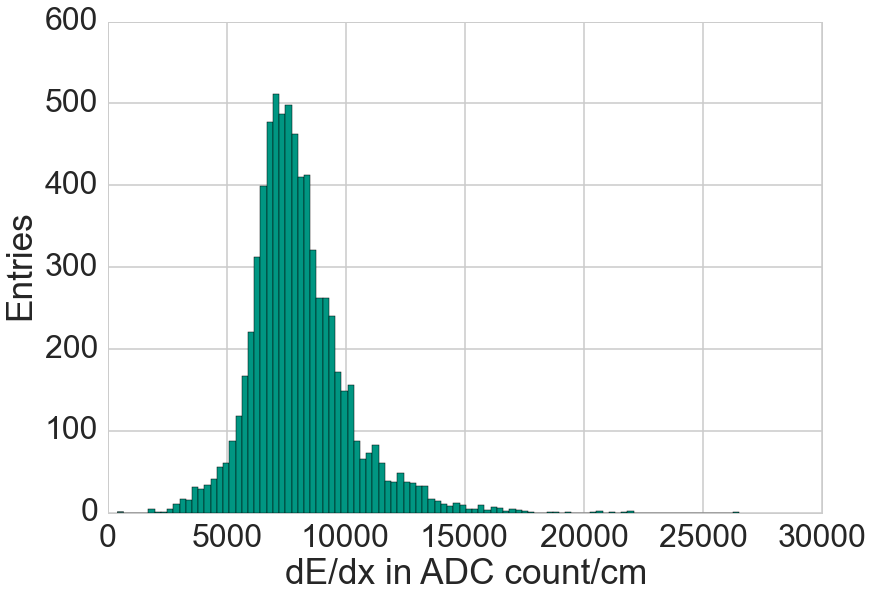
\includegraphics[width=0.7\linewidth]{figures/vxd/landau.png}
  \caption[Energy loss of particles in a sharp momentum range near of 70 MeV.]{Energy loss of particles in a sharp momentum range near of $\unit[70]{MeV}$. The distribution spreads over a large area in the \dedx space which causes the fit of the momentum estimation function to the full data to fail.}
  \label{fig-landau}
\end{figure}

\begin{figure}
  \centering
  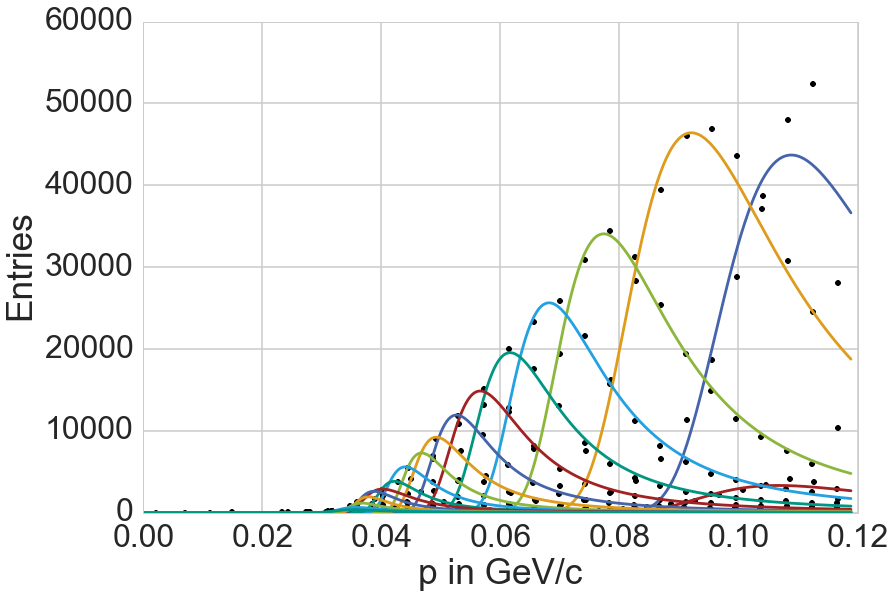
\includegraphics[width=0.48\linewidth]{figures/vxd/fitLandau1.png}
  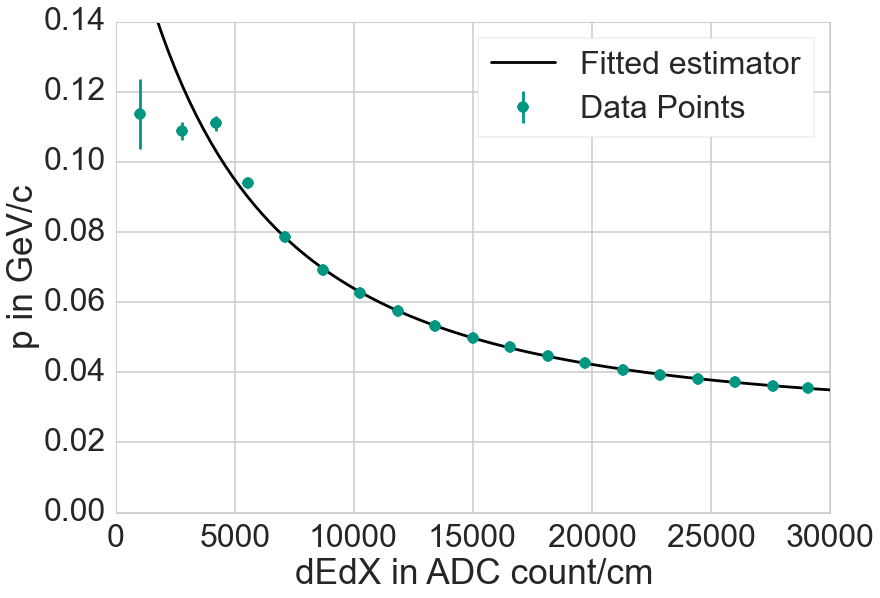
\includegraphics[width=0.48\linewidth]{figures/vxd/fitLandau2.png}
  \caption[The process of obtaining the estimator function $p(\mathrm d E/\mathrm d x)$.]{The process of obtaining the estimator function $p(\mathrm d E/\mathrm d x)$. The left picture shows the p-distributions for 15 \dedx bins. Each of the distributions get fitted by a landau distribution. The right plot shows the location parameter of these fitted landau distributions. These values are then used to fit the model in equation (\ref{form-model}).}
  \label{fig-fit-bins}
\end{figure}

For the incorporation of the gained momentum estimation into the helix fit of genfit, not the momentum value directly but $q/p$ is needed. This is why in the following the residuum of $p^{-1}$ instead of $p$ is presented.

In the two subplots of figure \ref{fig-divp-residuum} the median and the interquartile range of the residuum of the estimated to the MC momentum is shown. As both fit functions (normal and landau) lead to quite large shifts in the median, indicating a biased momentum estimation a correction procedure is introduced: a cubic polynomial is fitted to the median values which is later subtracted from the momentum estimation. These corrected estimators are also shown in the figure. They do reduce the median of the residuum but increase the interquartile range in turn.

\begin{figure}
  \centering
   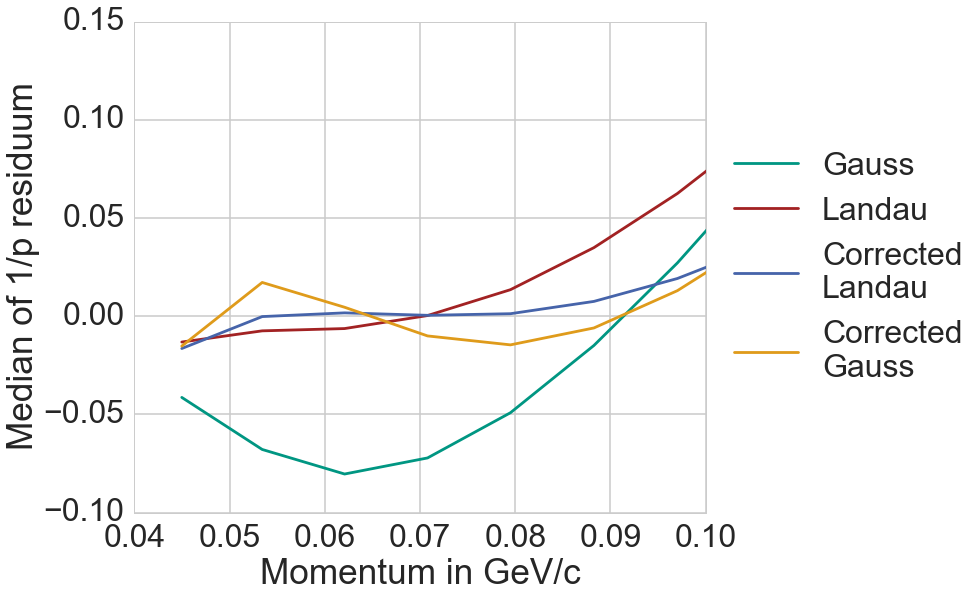
\includegraphics[width=0.47\linewidth]{figures/vxd/divPMedian.png}
   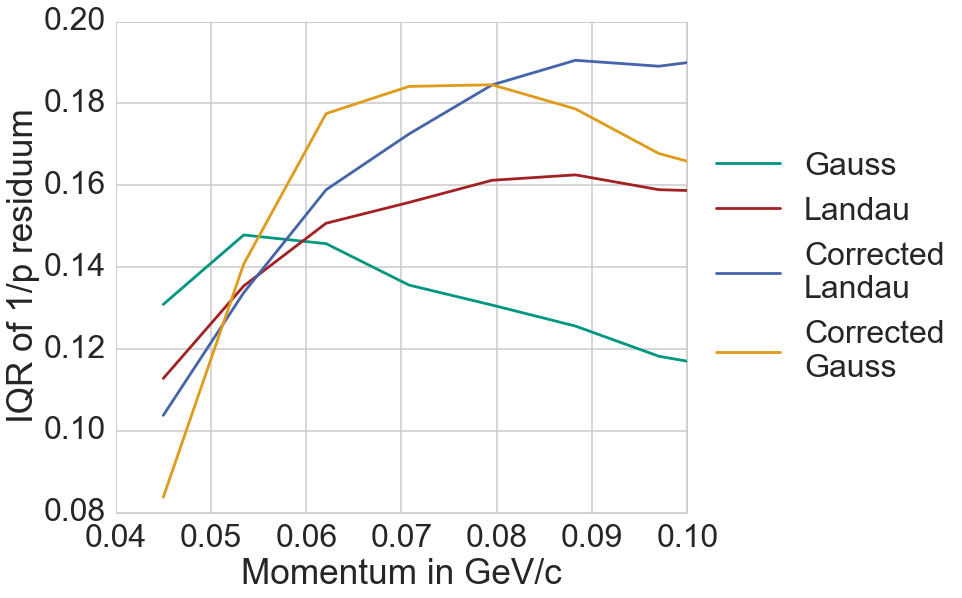
\includegraphics[width=0.47\linewidth]{figures/vxd/divPIQR.png}
  \caption[Median and IQR of $1/p$.]{The median (left) and the interquartile range (right) of the residuum between $1/p$ calculated with the estimator function and the MC information over the MC momentum. For all path length calculations the MC information at the hit is used. Together with the two fit functions landau and normal distribution also the median-corrected estimators (as described in the text) are shown.}
  \label{fig-divp-residuum}
\end{figure}


Besides the here presented two methods to gain the estimator function $p(\mathrm dE/\mathrm dx)$, also other fit models instead of equation (\ref{form-model}), other fit functions instead of landau and normal distribution and totally different methods like a boosted decision tree for regressions were tested. As all of these methods show worse results, they are not presented here. They can be easily compared to the mentioned results by using the IPython notebooks written by the author of this thesis.

\section{Incorporation in the helix fit}

Before describing the results of the momentum resolution with and without the new momentum estimation, the incorporation of this new measurement type is described shortly. For this, the measurement model used in genfit is summarized here briefly. More information can be found elsewhere~\cite{genfit}.

The idea of the genfit package as a generalized track fitting package is to not rely on a certain detector configuration but rather threat the measured hits in a general form. For this, every hit is transformed into a derived class of an \texttt{AbsMeasurement}. This measurement can hold up to five general coordinate measurements, which are two local coordinates $u$ and $v$, two local direction coordinates $u'$ and $v'$ and a coordinate for $q/p$. The measurement stores also the errors and covariances of these measurements and a generalized plane one which the measurements and the local coordinates are defined. The user does not have to provide all coordinate measurement in every \texttt{AbsMeasurement}. This general scheme makes it possible to incorporate all different results of the measuring detectors, e.g. VXD hits (which define a plane as the sensor plane and give one coordinate measurement of $u$ or $v$ for each strip in the case of SVD hits and both coordinates for PXD hits) or CDC wire hits (where the definition of a plane is more difficult to choose leading to a redefinition of the plane in every fit iteration). As the real detector measurements are uncoupled from the fitting algorithm, the implemented fitters do not have to be adopted to cope with different detectors.

To include the momentum estimation based on the \dedx value into the fit also, one has therefore to include another \texttt{AbsMeasurement} into the tracks for each VXD hit which is only filled with the $q/p$-coordinate and has the same plane as the positional measurement for this VXD hit. Another possibility would be to include this coordinate also in the already created positional measurements (by filling the two local positions $u$ and $v$ and the $q/p$ coordinate). The downside of this approach is that the DAF described in chapter \ref{chapter-theory} is then only able to downweight the whole measurement with the positional and the momentum coordinates and not the single measurement types only.

\subsection{Code basis for the fitting procedure}

While adding the momentum estimation to the VXD hits - but for other reasons also - the whole fitting framework in basf2 was rewritten. The former \texttt{genfit::Track} and the \texttt{genfit::TrackCand} where merged into a \texttt{RecoTrack} based on the \texttt{genfit::Track} which suits better to the StoreArray-scheme of the framework. Together with the new \texttt{RecoTrack} also other modules for fitting had to be written. The former \texttt{GenFitter} module was split up into smaller modules, each handling a single task. In the following, only the \texttt{MeasurementCreatorModule} will be described. More information on the \texttt{RecoTrack} and the other modules can be found in chapter \ref{chapter-addon}.

The task of this module is to create the measurements for each hit added to the \texttt{RecoTrack} by the track finding algorithms. The measurements can then be used by the track fitting routine. The \texttt{MeasurementCreatorModule} does so by calling configurable \texttt{MeasurementCreator} objects on all hits which can create a measurement out of the hit and the \texttt{RecoTrack}. There are preconfigured \texttt{MeasurementCreator} classes for turning the found hits into normal positional measurements like it was done before by the \texttt{GenFitterModule}. To handle the configuration of these \texttt{MeasurementCreator} objects in an easier way, the design pattern of factories was used in the module. Each type of \texttt{MeasurementCreator} objects (for looping over SVD, PXD or CDC hits found by the track finder or for no underlaying track finder hit at all) has an \texttt{MeasurementCreatorFactory}. These factories handle the configuration and initialization of the \texttt{MeasurementCreator} objects which in turn create measurements and add them to the \texttt{RecoTrack}. The configuration of the factories can be done via dictionaries passed as module parameters in the steering files. The whole process is shown in figure \ref{fig-measurement-creator}.

\begin{figure}
  \centering
  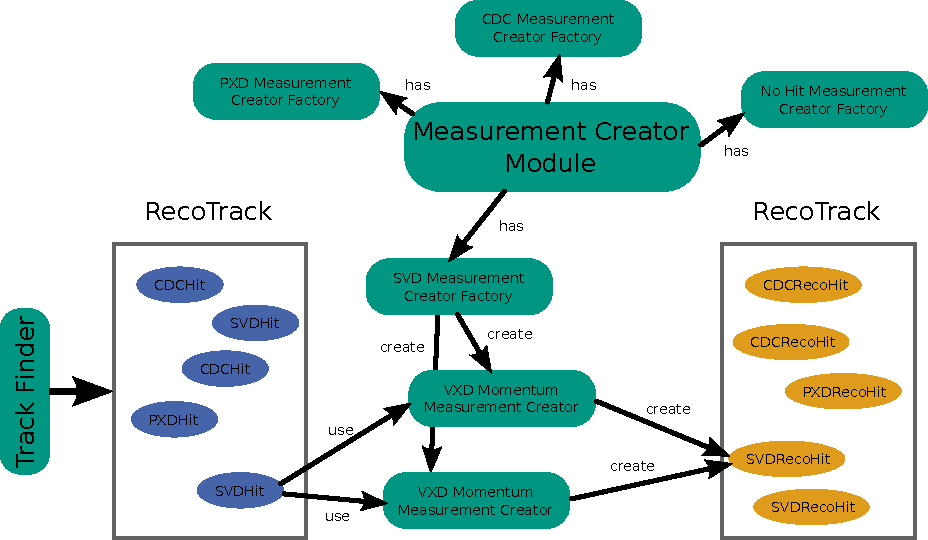
\includegraphics[width=\linewidth]{figures/vxd/measurementCreator.pdf}
  \caption[Diagram showing the creation of measurements.]{Diagram showing the creation of measurements in the \texttt{MeasurementCreatorModule} as described in the text. Each \texttt{RecoTrack} includes PXD, SVD and CDC hits (blue) added by the track finder algorithms which must be transformed into \texttt{AbsMeasurement} objects (orange) to be handled by the track fitting routine later. These measurements can include positional, directional and/or $q/p$ coordinate values with their errors.}
  \label{fig-measurement-creator}
\end{figure}

The momentum estimation of the VXD hits is included into the fit as another measurement - created also by a \texttt{MeasurementCreator} object. The measurements are created before the track fit but get called for their parameters in ever fitting iteration right before the fit uses the coordinates in the measurement. This fact can be used to calculate the plane (as used in the CDC hits) or the coordinates just before using them. Therefore it is possible to use the fitted state right in front of the hit to calculate the path length as described in subsection \ref{subsection-calc}. Together with the estimation for $q/p$ also the error on this coordinate has to be included into the \texttt{AbsMeasurement}. This error can be calculated using the MC momentum used for calculating the estimator function and comparing this to the estimator function result. The error is fixed to 0.3 in the moment, but can in principle be also calculated for every measurement independently.

\subsection{Resolution after track fitting}

The above described estimation is included as a \texttt{MeasurementCreator} for SVD and PXD hits and the pion tracks in the momentum range of 50 - 100 MeV are fitted using the Kalman filter. Then the momentum calculated in the fit is compared to the one used in the MC simulation. To show the resolution in an easier way, the median and the interquartile range for the residuum is calculated. They can be seen in figure \ref{fig-results-fit} for both fit functions landau and gauß (with their median-corrected estimators also) and for the different path length calculations in figure \ref{fig-results-fit2}.

\begin{figure}
  \centering
  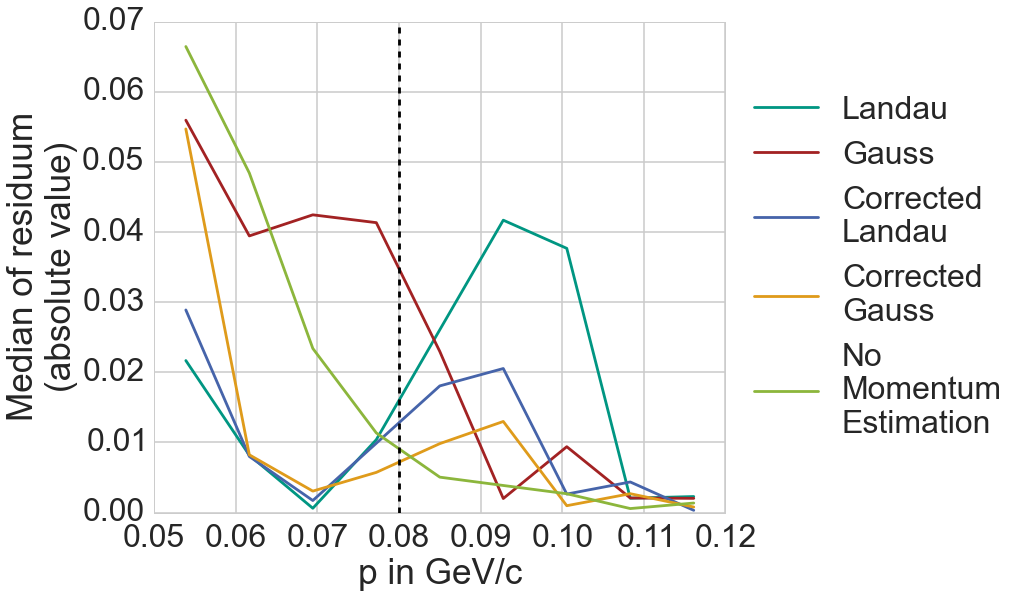
\includegraphics[width=0.48\linewidth]{figures/vxd/kalman0_3Median.png}
  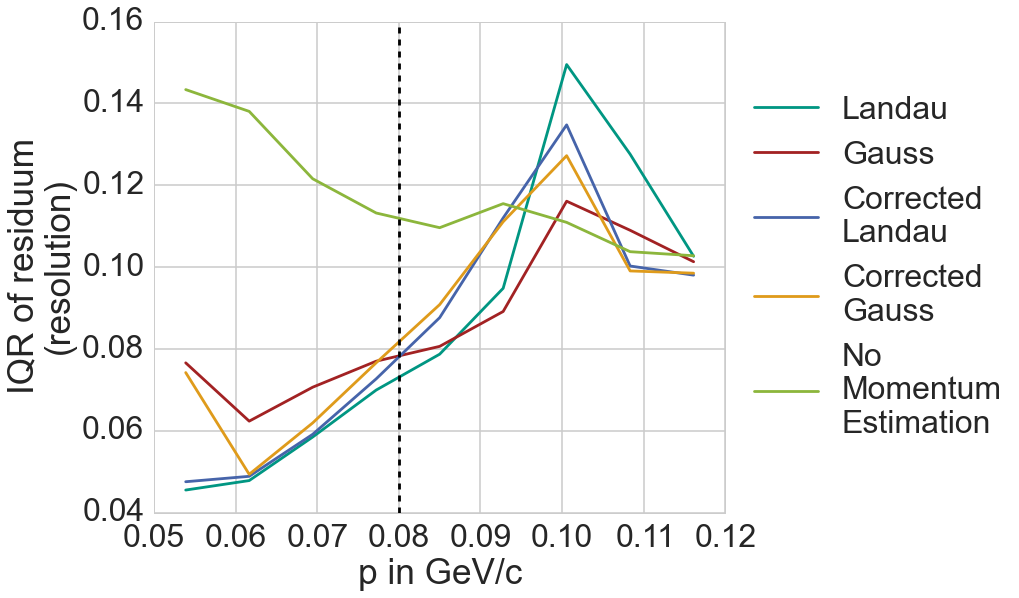
\includegraphics[width=0.48\linewidth]{figures/vxd/kalman0_3IQR.png}
  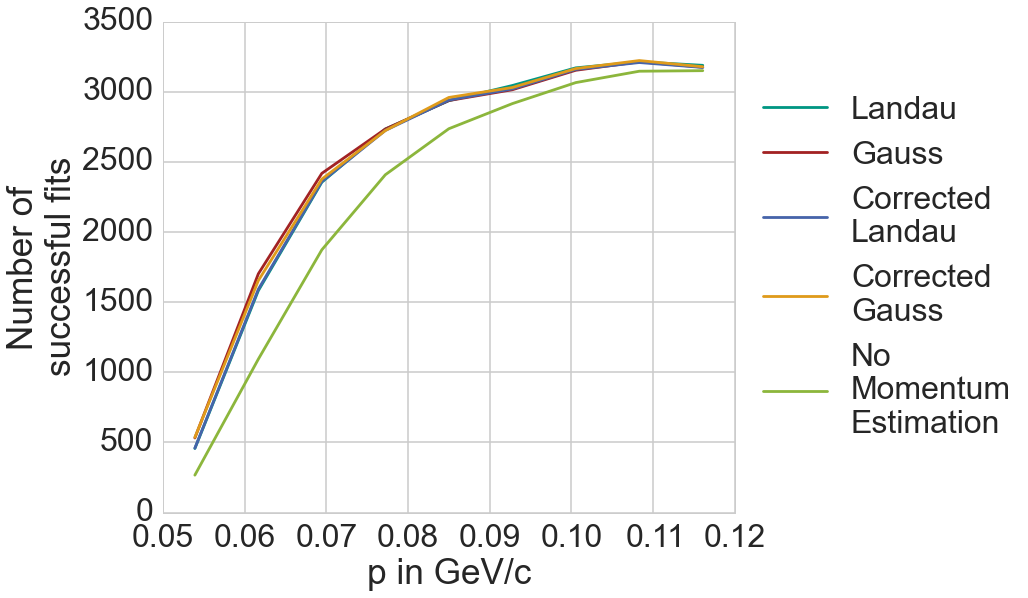
\includegraphics[width=0.48\linewidth]{figures/vxd/kalman0_3Count.png}
  \caption[Residuum of the momentum estimation for different fit functions.]{Figure showing the median (left) and the interquartile range (right) for the residuum between the MC momentum and the momentum coming from the helix fit with or without the momentum estimation based on the energy loss information. The two different fit functions landau and norm (like described in subsection \ref{subsection-transform}) are both shown here. The third plots shows the number of successful fits.}
  \label{fig-results-fit}
\end{figure}


\begin{figure}
  \centering
  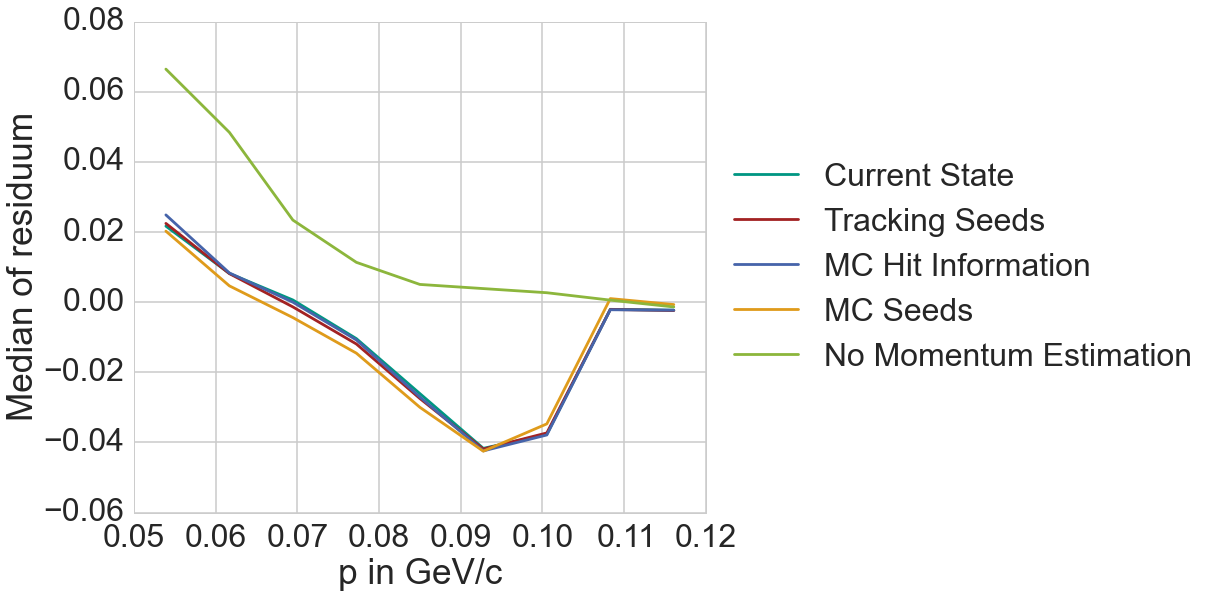
\includegraphics[width=0.48\linewidth]{figures/vxd/landauKalman0_3Median.png}
  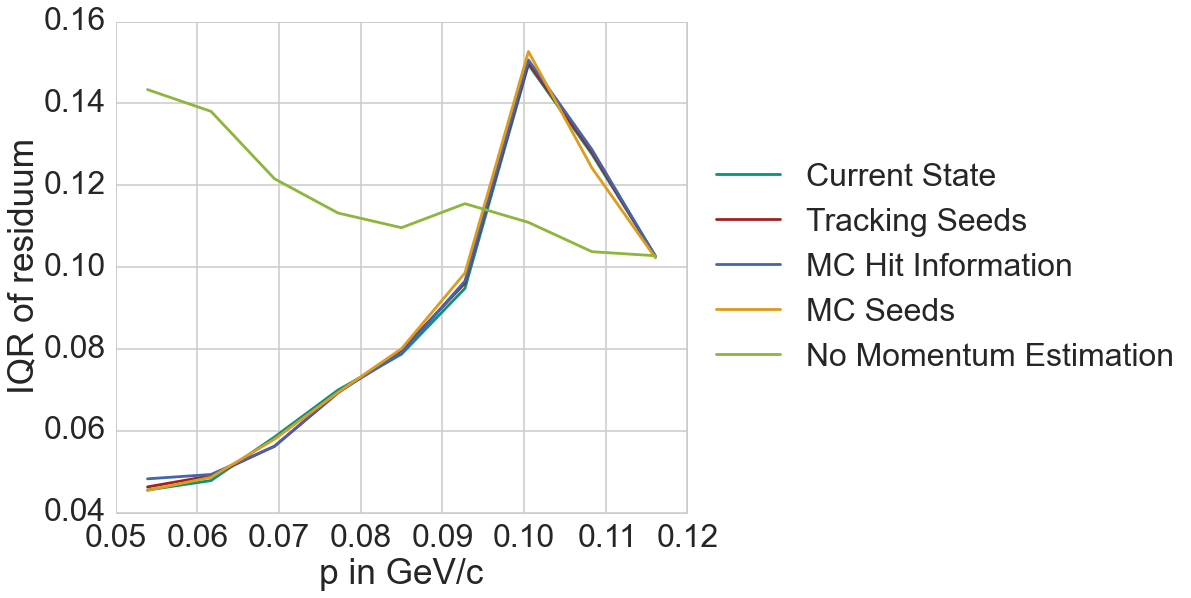
\includegraphics[width=0.48\linewidth]{figures/vxd/landauKalman0_3IQR.png}
  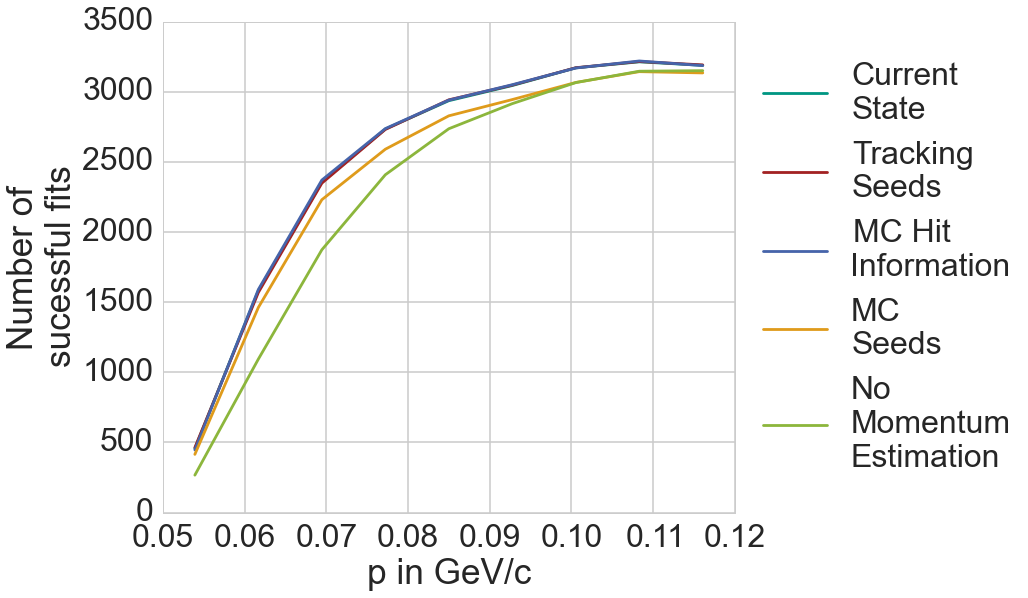
\includegraphics[width=0.48\linewidth]{figures/vxd/landauKalman0_3Count.png}
  \caption[Residuum of the momentum estimation for different path length calculations.]{Figure showing also the median (left) and the interquartile range (right) of the residuum and the number of successful fits as in figure \ref{fig-results-fit}. This time the different path length calculations are shown for the case of using a landau distribution for fitting the \dedx values.}
  \label{fig-results-fit2}
\end{figure}

As it can be seen in the result figures, the incorporation of the VXD momentum estimation into the helix fit can increase the resolution of the momentum quite drastically for low momentum tracks while also increasing the number of successful fits. As the landau seems to perform slightly better than the gauß fitted estimator function, these values are used in the following. Although the median-corrected functions should theoretically behave better, the resolution could not be increased. This may come from the worsen interquartile range of the corrected estimators as seen in figure \ref{fig-divp-residuum}. The differences between the different path length calculations are not that big as expected from the prestudies of the path lengths before. As described before, the calculation with the MC track parameters at the hit perform best followed by the track parameters at the hit while fitting. The differences are very small as the fitted parameters and the MC parameters are similar enough. For momenta above 100 MeV the estimator gives worse results as it can be also seen in figure \ref{fig-dedx-over-p}. This is why the momentum resolution deteriorates for higher momenta. There is already a cut for only applying the momentum estimation for low-momenta-tracks, but because of implementation details in the genfit package this cut can only be evaluated before the fit - so using the track finder seed parameters. As these parameters often underestimate the momentum (because of energy losses due to material effects), the momentum estimation gets applied although the estimator is not build for this momentum region. To solve this problem, a ``smarter'' cut should be introduced.

Besides the momentum resolution, the resolution of the other helix parameters should not be decreased by the momentum estimation measurements. The perigee position of the fitted tracks with and without the momentum estimation with the landau fit function and path lengths from the track fit state is shown in figure \ref{fig-position}. As all tracks where simulated using a particle gun at the origin, the position should be exactly zero. For better comparison with the typical validation plots shown in the collaboration, the VXD and CDC tracks are merged and fitted together. As it can be seen in the picture, the resolution in the position is reduced by introducing the momentum estimation into the fit. One reason for this is probably the neglected correlation between the momentum estimation and the position measurement. Another issue is the fixed error of the momentum estimation, which can bias the fit. The resolution in the $z$ coordinate stays equally good - only the $x$ and $y$ coordinates are affected. Further analysis must be done to increase the resolution of the perigee position again.

\begin{figure}
  \centering
  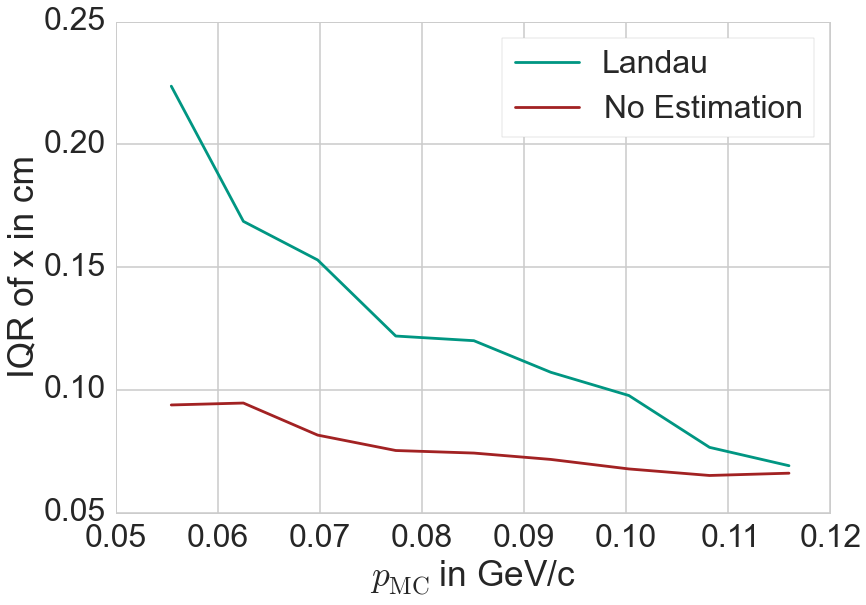
\includegraphics[width=0.48\linewidth]{figures/vxd/perigee_x.png}
  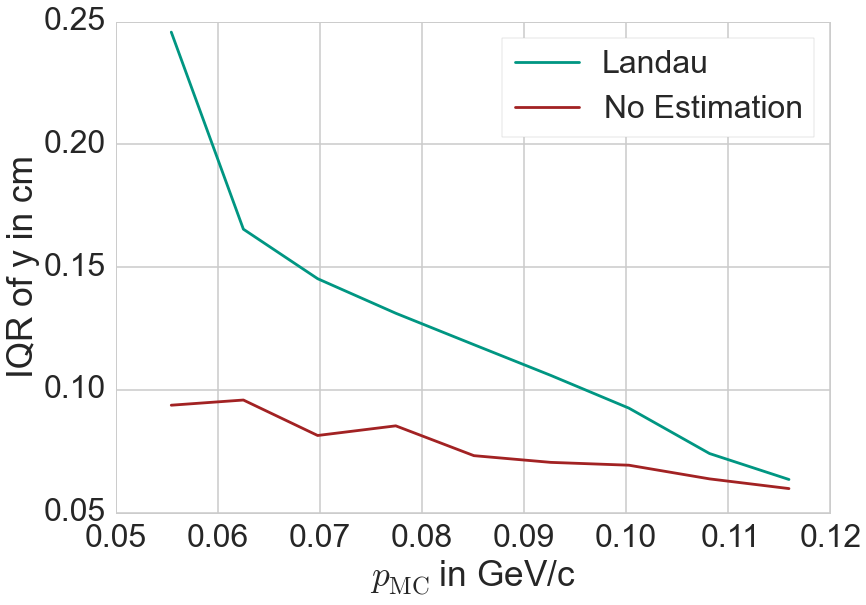
\includegraphics[width=0.48\linewidth]{figures/vxd/perigee_y.png}
  \includegraphics[width=0.48\linewidth]{figures/vxd/perigee_z.png}
  \includegraphics[width=0.48\linewidth]{figures/vxd/perigee_r.png}
  \caption[Perigee position with and without the momentum estimation.]{The IQR of the position at the perigee resulting from the helix fit with and without the momentum estimation. As the MC position is exactly zero, a residuum can not be calculated properly. The value of $r$ is calculated using $r=\sqrt{x^2 + y^2}$}
  \label{fig-position}
\end{figure}

% the pull distribution of the momentum and the three position resolutions is calculated and shown in figure \ref{fig-pull}. \todo{Beschreibung}

% \begin{figure}
%   \centering
%   \includegraphics[width=0.48\linewidth]{figures/vxd/pullMomentum.pdf}
%   \includegraphics[width=0.48\linewidth]{figures/vxd/pullPositionX.pdf}

%   \includegraphics[width=0.48\linewidth]{figures/vxd/pullPositionY.pdf}
%   \includegraphics[width=0.48\linewidth]{figures/vxd/pullPositionZ.pdf}
%   \todo{picture}
%   \caption[Pull distributions for the total momentum and the three coordinates of the perigee.]{Pull distributions for the total momentum and the three coordinates of the perigee. TODO: Beschreibung}
%   \label{fig-pull}
% \end{figure}

The next analysis is concerning the errors included into the momentum measurement. As the error is included as a fixed value for all momenta, it is not expected to be correct. Nevertheless the p-value of the whole track fit is presented in figure \ref{fig-p-values} with and without the VXD momentum estimation again with CDC and VXD tracks merged. The error introduced in the new measurement seems to be underestimated which causes the p-value to shift to smaller values. This can be caused by the fixed value of the error for all momenta (which is definitely wrong as the residuum distribution behaves differently for different momenta as seen in figure \ref{fig-results-fit}). Another reason is the distribution of \dedx for a fixed momenta - a landau distribution - which has a long tail towards higher energy losses and can therefore not be described well by a gaussian distribution (which must be used to calculate the error in genfit). Here is probably much room for improvement in further developments.

\begin{figure}
  \centering
  \includegraphics[width=0.7\linewidth]{figures/vxd/pValue.png}
  \caption[P-values of the whole track fit]{P-values of the whole track fit with and without the VXD momentum estimation for merged CDC and VXD tracks with the landau fit function and path lengths calculated with the current fit state. The p-value is much lower with the VXD momentum estimation indicating underestimated errors introduced in the fit.}
  \label{fig-p-values}
\end{figure}


\section{Conclusion and further possibilities}

By introducing a new measurement type into the fit of VXD tracks using a generated momentum estimator function and the \dedx value, the resolution of the momentum after the fit could be increased for low momenta tracks. The handling of the error of this measurement and the correlations to the other coordinates (especially the local position coordinates) must be further analyzed to enhance the position information and the p-values again. Also a better handling of the decision when to apply the momentum estimation should be included. The \texttt{MeasurementCreator} and the measurement type of the VXD momentum estimation should be constructed in such a way to handle these improvements.

A different approach was used in other experiments~\cite{sergey}: the fitting algorithm calculates the energy loss in every sensor when handling the material effects in every fit step. This energy loss can be compared to the one measured by the sensors and the fit parameters can be corrected. This method has the benefit of not needing a momentum estimator function for transforming the \dedx value to a momentum estimation as it uses the raw \dedx information. It also does not need to calculate the path length by using a helix parametrization but uses the step length in every fit step. The downside of this approach is, that it relies on a correctly calibrated measured energy loss in the sensor with which it can compare. Another disadvantage is that the energy loss measurement can not be handled in the same way as the other measurements and there is no possibility to downweight it in the DAF algorithm or include the correlation to the coordinate measurements. When it comes to the underestimated error because of the landau tail and the condition when to include this momentum estimation, this approach shares the same problems as the here presented.


  \chapter*{Summary}

As described in the introduction, the track finding plays a crucial role for the physics analyses performed on the data to be taken by the planned Belle~II experiment. The need for very high finding efficiencies and also high purities make a severe demand on the tracking algorithms which should additionally be fast and configurable.

Within the scope of this thesis, the algorithms for the tracking in the central drift chamber (CDC) detector were analyzed, refined or newly developed. The stereo hit finder and the module combining segments from the local and tracks from the global finder as well as tools for improving the track quality were firstly built during this work. The performed changes could improve the number of found tracks and hits, the rate of fitted tracks and also the computing time significantly.

Together with the improvements on the tracking figures of merit some parts of the Legendre track finding software was reworked and adapted to modern programming styles and a common code basis. As this thesis was the first to evaluate the track finding package in the CDC, several errors in the software were corrected and the validation features were improved. Additionally, the modularity of and the connectivity between the tracking modules for the CDC detector was increased, which made it easier to try out new possibilities and approaches for combining the track finders. Also, this thesis was the first to summarize the characteristics of the CDC track finding algorithms to give additional hints where there is room for improvements. Some of these improvements have already been implemented into the software.

The last step in the tracking procedure -- the track fitting -- still imposes some sever problems to the track finding in the CDC detector which have to be solved before the start of the experiment. After that, the influence of the various particle properties on the track finder has to be analyzed in order to optimize the algorithms to their later use case. As all shown figures of merit rely on the correctness of the event and the background Monte Carlo simulation, these have to be checked and possibly corrected in the early phases of the experiment.

Another part of this thesis consisted of a first analysis of incorporating the $\mathrm dE/\mathrm d x$ value as another measurement into the trajectory fit for low momentum tracks in the vertex detectors to improve the momentum resolution. An estimator for calculating the momentum with the energy loss for each hit individually was developed and different possibilities to do so were compared. The estimation was then inserted into the fitting procedure with configurable parameters. The momentum resolution and the number of successful fits for momenta below $\unit[80]{MeV}$ could be increased drastically. Further developments and studies to improve the error estimation and the transverse position resolution should be performed. Therefore, the newly created track class and the additional modules are easy to extend and can handle further changes.

% Also, some new functionalities as the \texttt{ipython\_handler} or the \texttt{root\_pandas} module in the software framework and the \texttt{RecoTrack} data structure in the tracking package were implemented.

The refined tracking algorithms -- especially for the CDC detector -- which were partly developed in the thesis are expected to improve the figures of merit of the tracking in the Belle~II detector. They have therefore a strong influence on all analyses which will be performed on the taken data. The combination of the two track finders improved the number of correctly added hits of the found tracks. All in all, a significant improvement over the reference implementation is seen in the figures of merit and also in the computing time which opens a wide window of new possibilities for refined physics analyses.

  % Anhang
  \chapter*{Danksagung}
\begin{otherlanguage}{ngerman}
Zum Abschluss möchte ich allen danken, die zur Fertigstellung dieser Arbeit beigetragen haben.

Zuallererst danke ich Prof. Dr. Michael Feindt für die Möglichkeit diese Masterarbeit schreiben zu können und seine Förderung darüber hinaus.

Vielen Dank auch an Prof. Dr. Ulrich Husemann für die Übernahme des Korreferats.

Bei Dr. Martin Heck und Dr. Thomas Hauth möchte ich mich sehr für die allzeit gute und umfassende Betreuung und Unterstützung bedanken.

Das offene und kreative Arbeitsumfeld in der Arbeitsgruppe hat mir sehr geholfen. Insbesondere Christian Pulvermacher und Markus Prim möchte ich für ihre Hilfe danken. Dank gilt auch dem Admin-Team des EKP, ohne welches meine Arbeit so sicherlich nicht möglich gewesen wäre.

Schließlich möchte ich meiner Familie und meinen Freunden danken, welche mich immer unterstützt haben und auf die ich mich verlassen konnte.
\end{otherlanguage}
  \appendix
  \bgroup\let\addcontentsline=\nocontentsline\listoffigures\egroup  
\bgroup\let\addcontentsline=\nocontentsline\listoftables\egroup
\bgroup\let\addcontentsline=\nocontentsline\listoflistings\egroup

\bibliographystyle{class/utphys}
\bgroup\let\addcontentsline=\nocontentsline\bibliography{class/bibliography}\egroup

  \bgroup\let\addcontentsline=\nocontentsline\listoffigures\egroup  
  \bgroup\let\addcontentsline=\nocontentsline\listoftables\egroup

  \bibliographystyle{class/utphys}
  \bgroup\let\addcontentsline=\nocontentsline\chapter{Bibliography}\egroup
  \bibliography{class/bibliography}

\end{document}
